%   \label{sec:signalIndependentLimits}% uncomment if label used. 
\subsubsection{Untagged Resonances: Model-independent Gaussian Limits}
%       \label{subsec:UntaggedResonancesGaussianLimits} % uncomment if label used. 
One way to demonstrate the search in the analysis is to set limits on the cross-section of signal modes. Here a model-independent signal as Gaussian are used to expand the sensitivity of the search to new signals that may be detectable with this analysis but not currently theoretically described. Besides, a model-independent signal could help to evaluate and compare the strength of different analyses without bias, as the case where specific models are applied and leads less sensitive to the search.

Therefore, model-independent limits are produced based on model-independent signal resonances. Because this analysis is sensitive to the shape of resonance, specific models with different shapes would influence the results strongly. In general, a model-independent signal is a good feature of the analysis which verify the ability to distinguish different signal models, although the model-independent limits are still influenced by the shape of the resonance in an implicit way. The motivation to choose a Gaussian resonance as a proxy is the fact that it is similar to the `average' signal with specific width. Besides, the shape of reconstructed jet \pt~of any realistic signal without very specific model is produced approximately as a Gaussian resonance, without applied JER. Hence it it straightforward to use Gaussian resonances to represent any realistic resonance:


The untagged $y^{*} < 0.8$, 1-$g$ tagged $y^{*} < 0.6$ and 2-$g$ tagged $y^{*} < 0.8$ model-independent Gaussian limits are shown in fig \ref{fig:SignalIndependentGaussianLimits_UntaggedYStar0p8}, \ref{fig:SignalIndependentGaussianLimits_1gYStar0p6} and \ref{fig:SignalIndependentGaussianLimits_2gYStar0p8} respectively, for Gaussians with width equal to 0, 3, 5, 7, 10 and 15\% of their peak position, without systematics included. 

        \begin{figure}[!htb]
            \subfloat[0\% Width Gaussian Limits]{ 
%                \label{fig:SignalIndependentGaussianLimits_SubWidth0} % uncomment if label used. 
                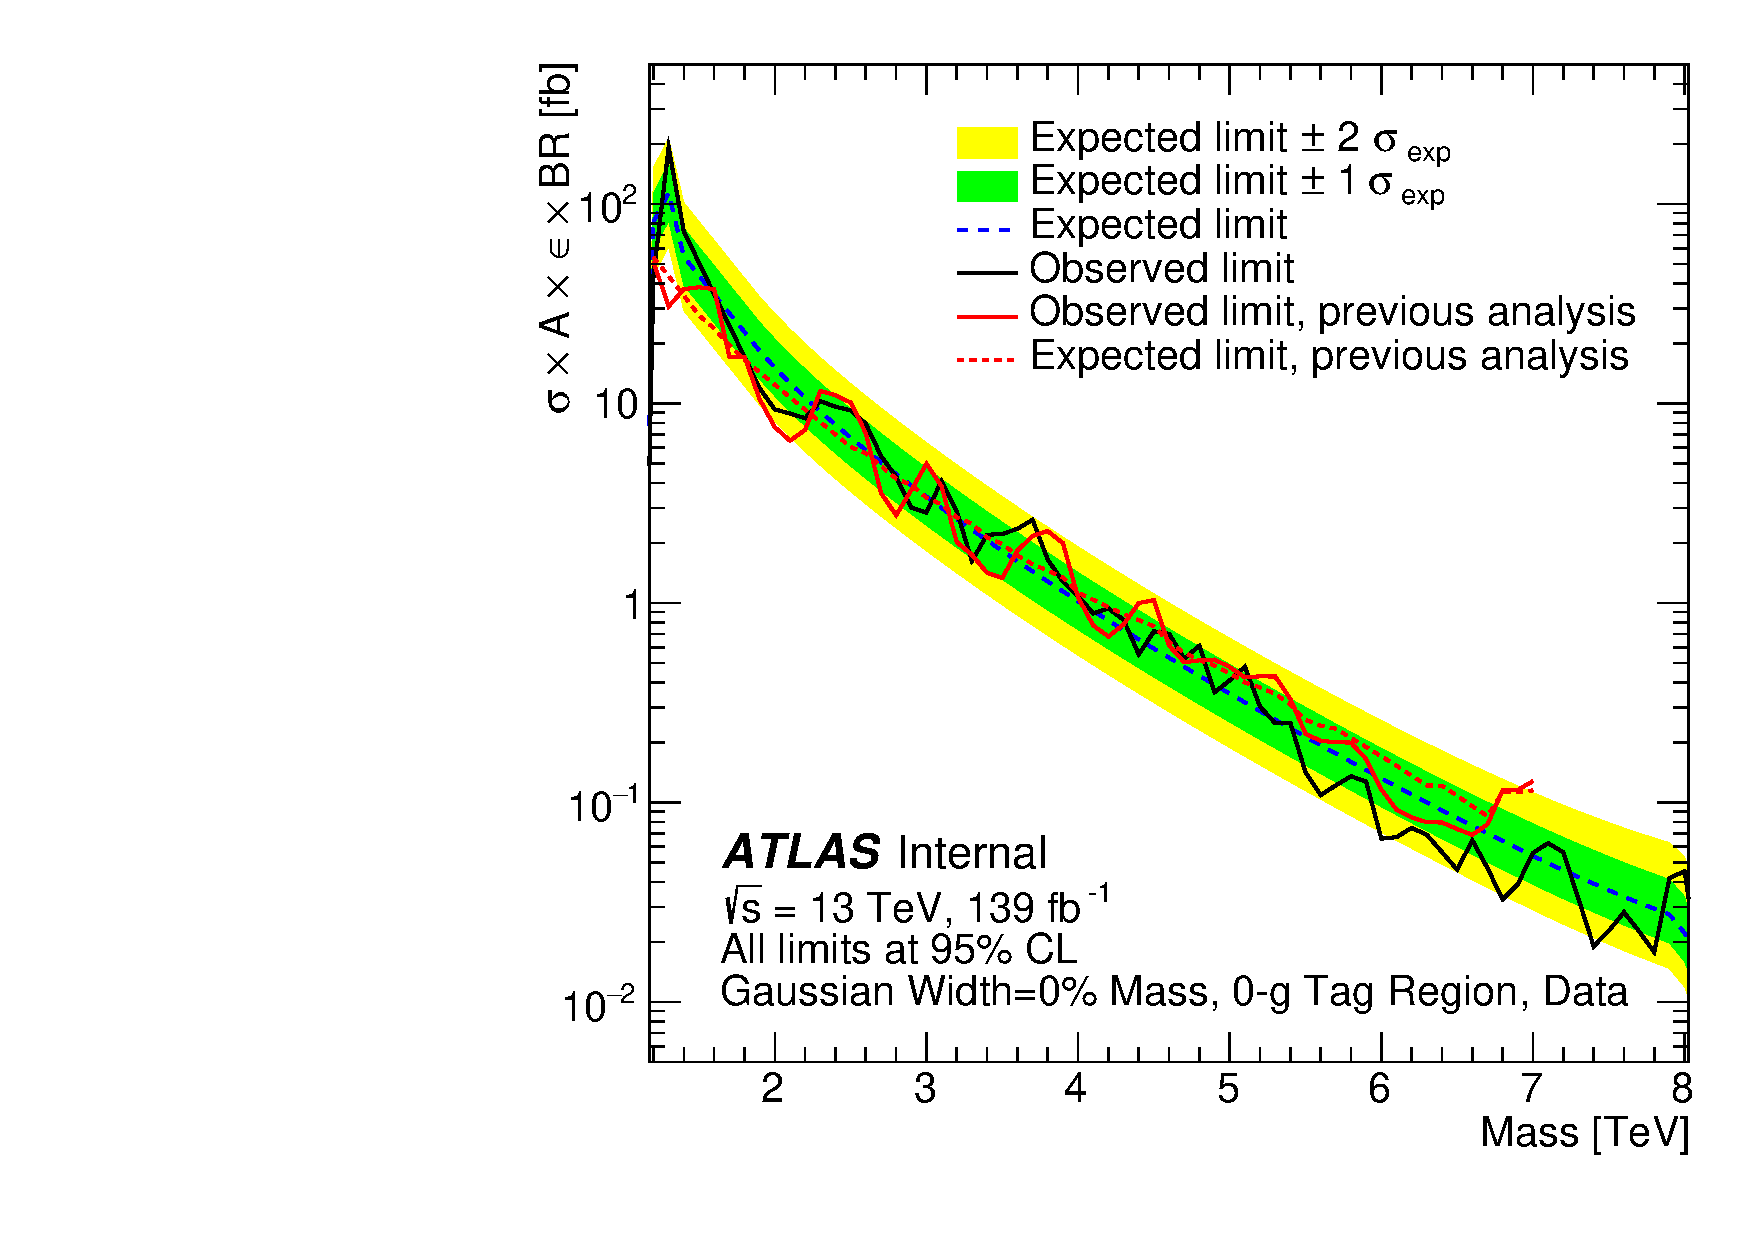
\includegraphics[width=0.4\textwidth]{fig/app-SignalIndependentLimits/Gauss_Limits_yStar0p8_Tag0_WidthPercent0_1200to8000_sigma.pdf}
            }
            \subfloat[3\% Width Gaussian Limits]{ 
%                \label{fig:SignalIndependentGaussianLimits_SubWidth3} % uncomment if label used. 
                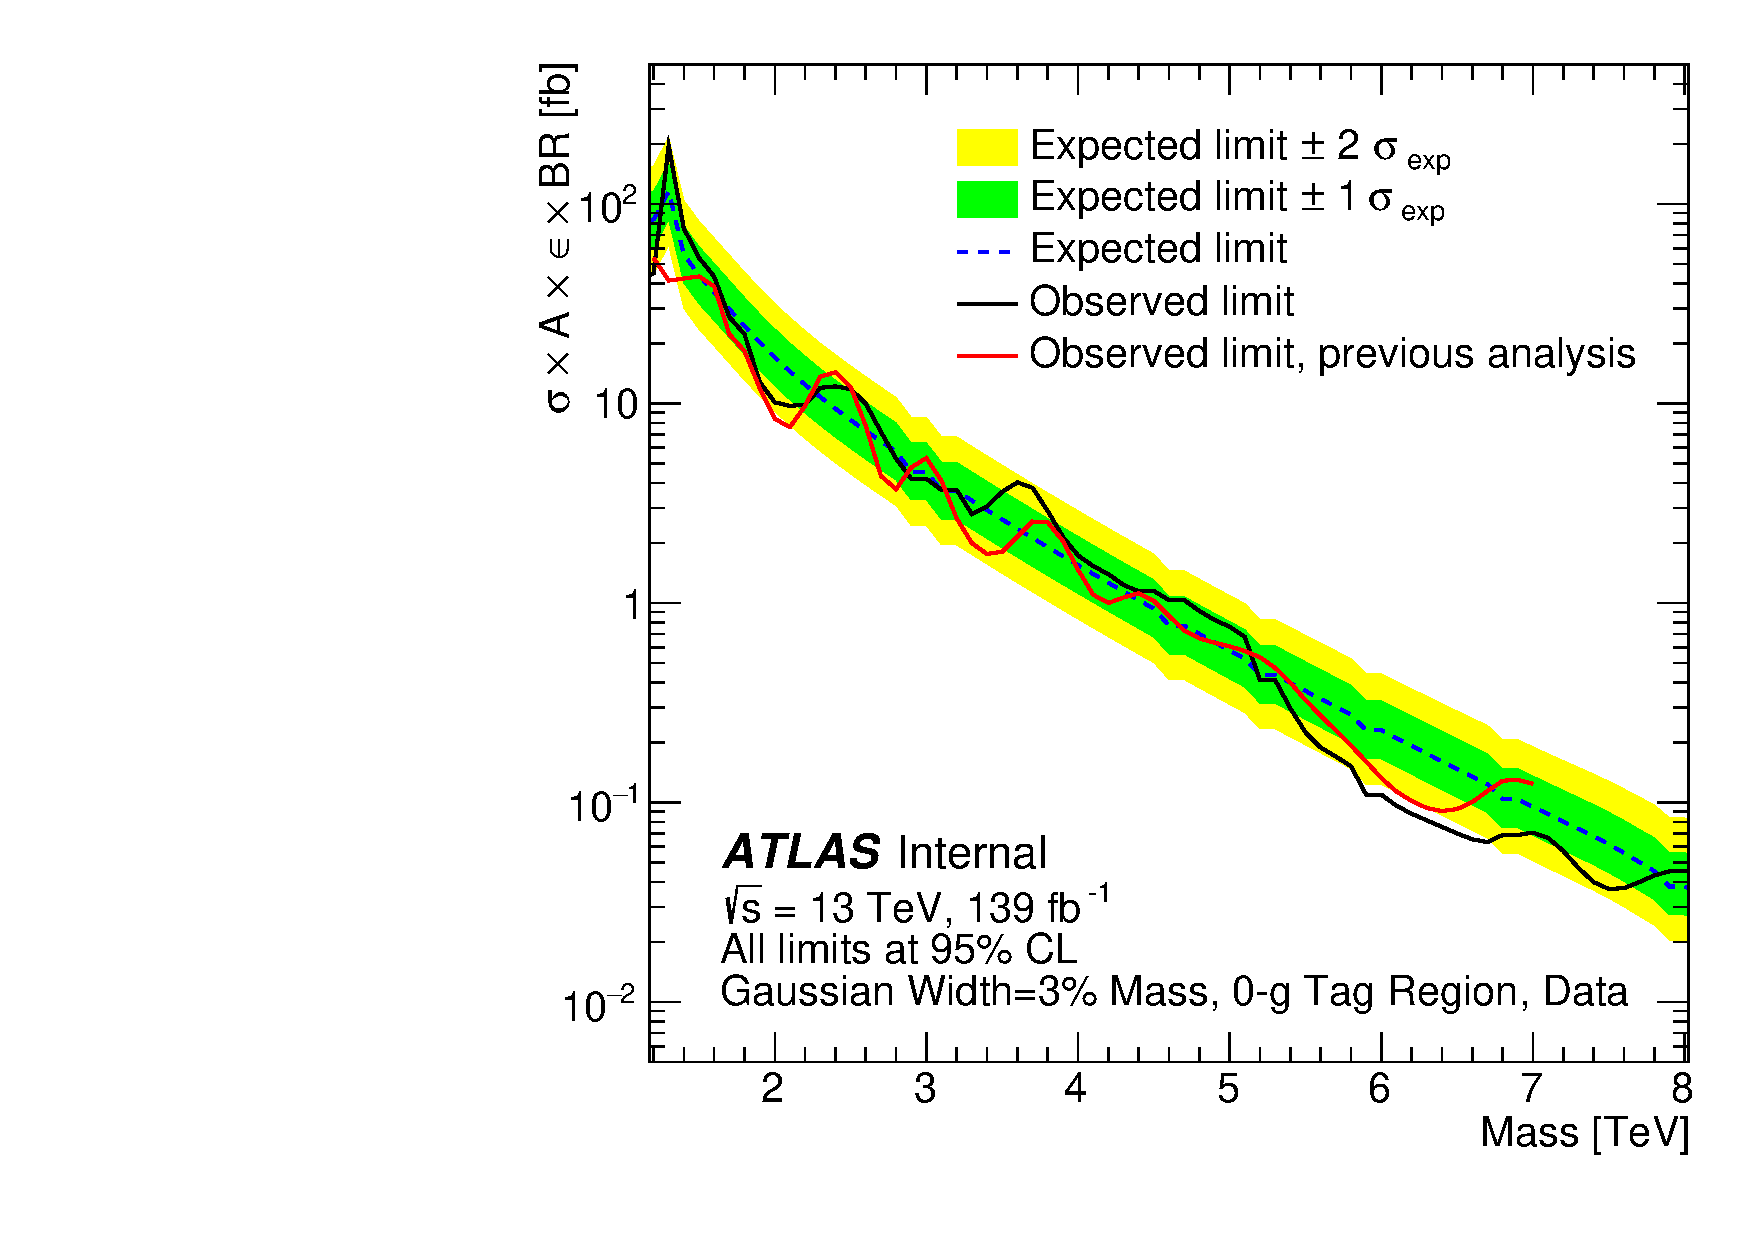
\includegraphics[width=0.4\textwidth]{fig/app-SignalIndependentLimits/Gauss_Limits_yStar0p8_Tag0_WidthPercent3_1200to8000_sigma.pdf}
            }\\
            \subfloat[5\% Width Gaussian Limits]{ 
%                \label{fig:SignalIndependentGaussianLimits_SubWidth5} % uncomment if label used. 
                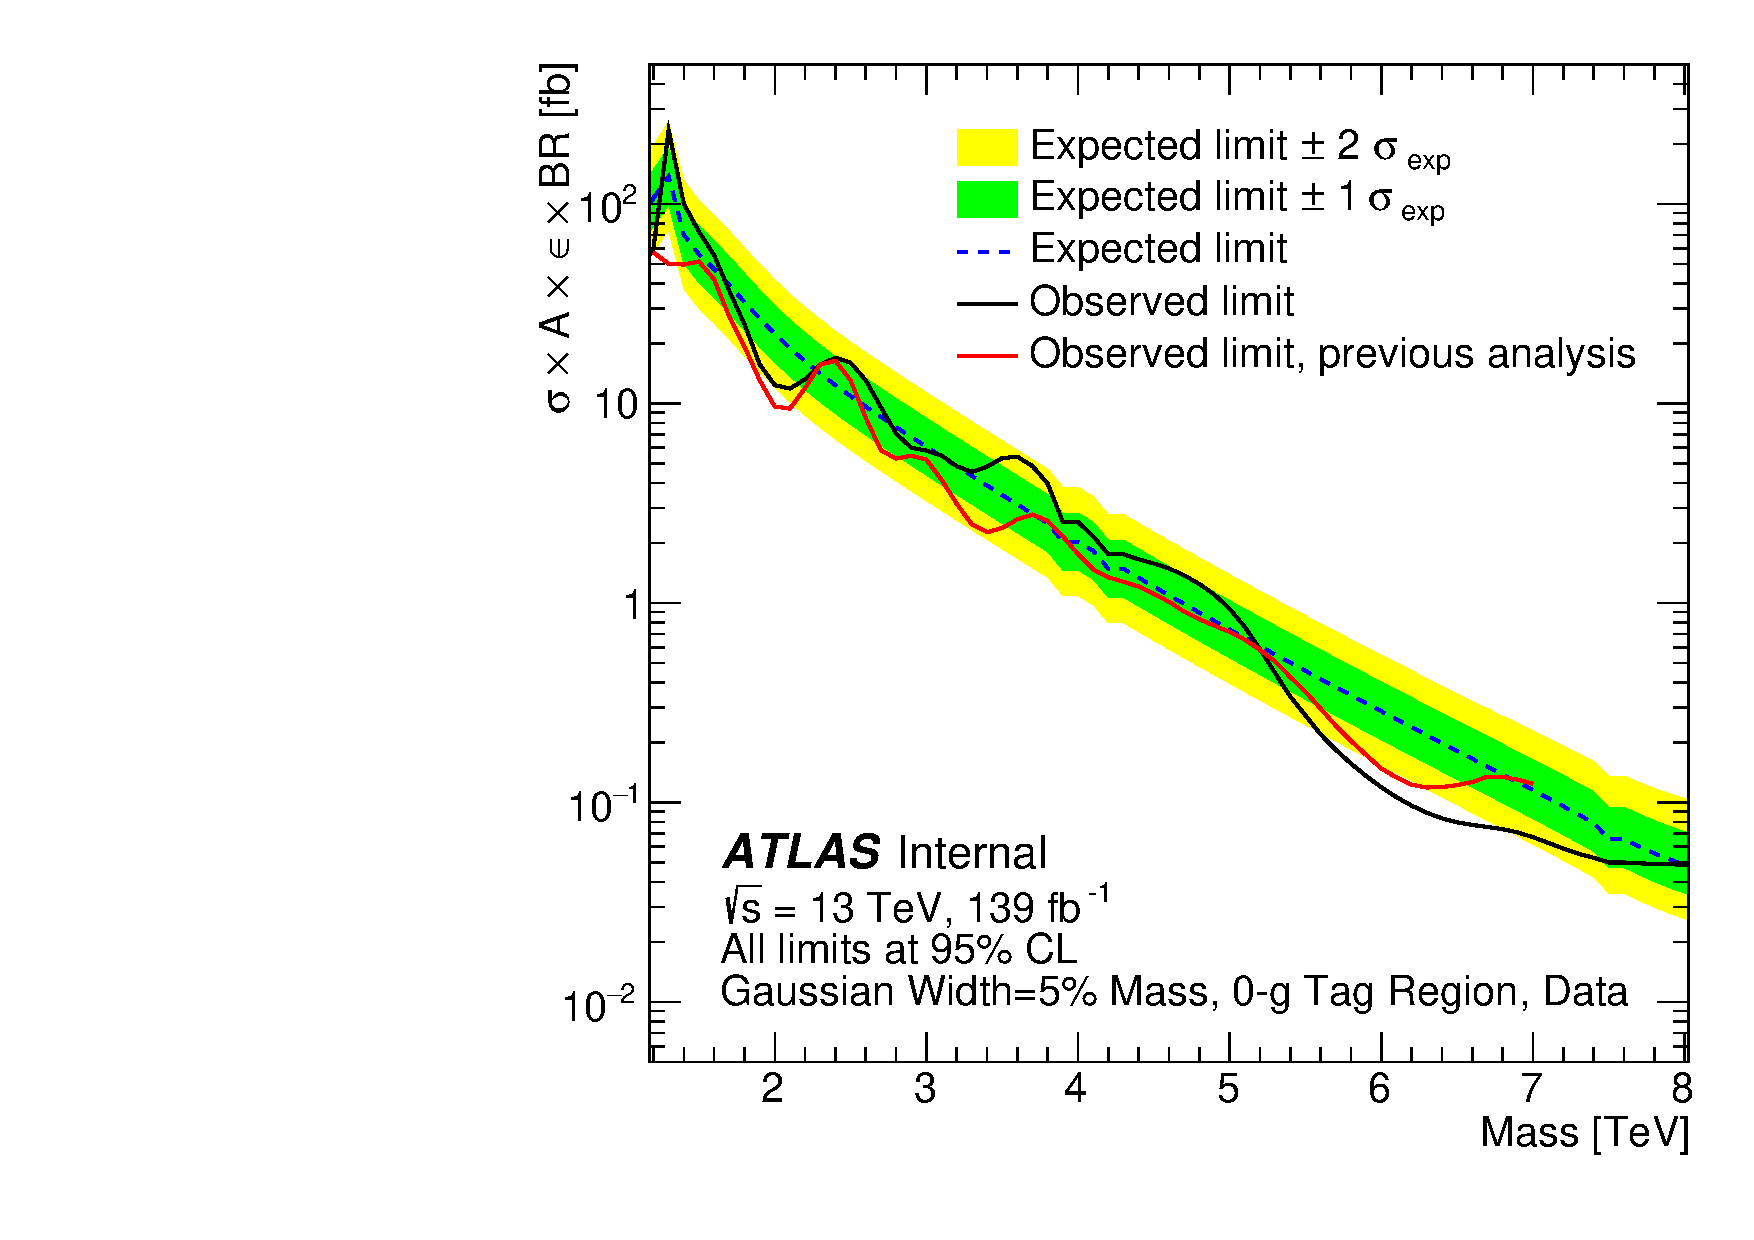
\includegraphics[width=0.4\textwidth]{fig/app-SignalIndependentLimits/Gauss_Limits_yStar0p8_Tag0_WidthPercent5_1200to8000_sigma.pdf}
            }
            \subfloat[7\% Width Gaussian Limits]{ 
%                \label{fig:SignalIndependentGaussianLimits_SubWidth7} % uncomment if label used. 
                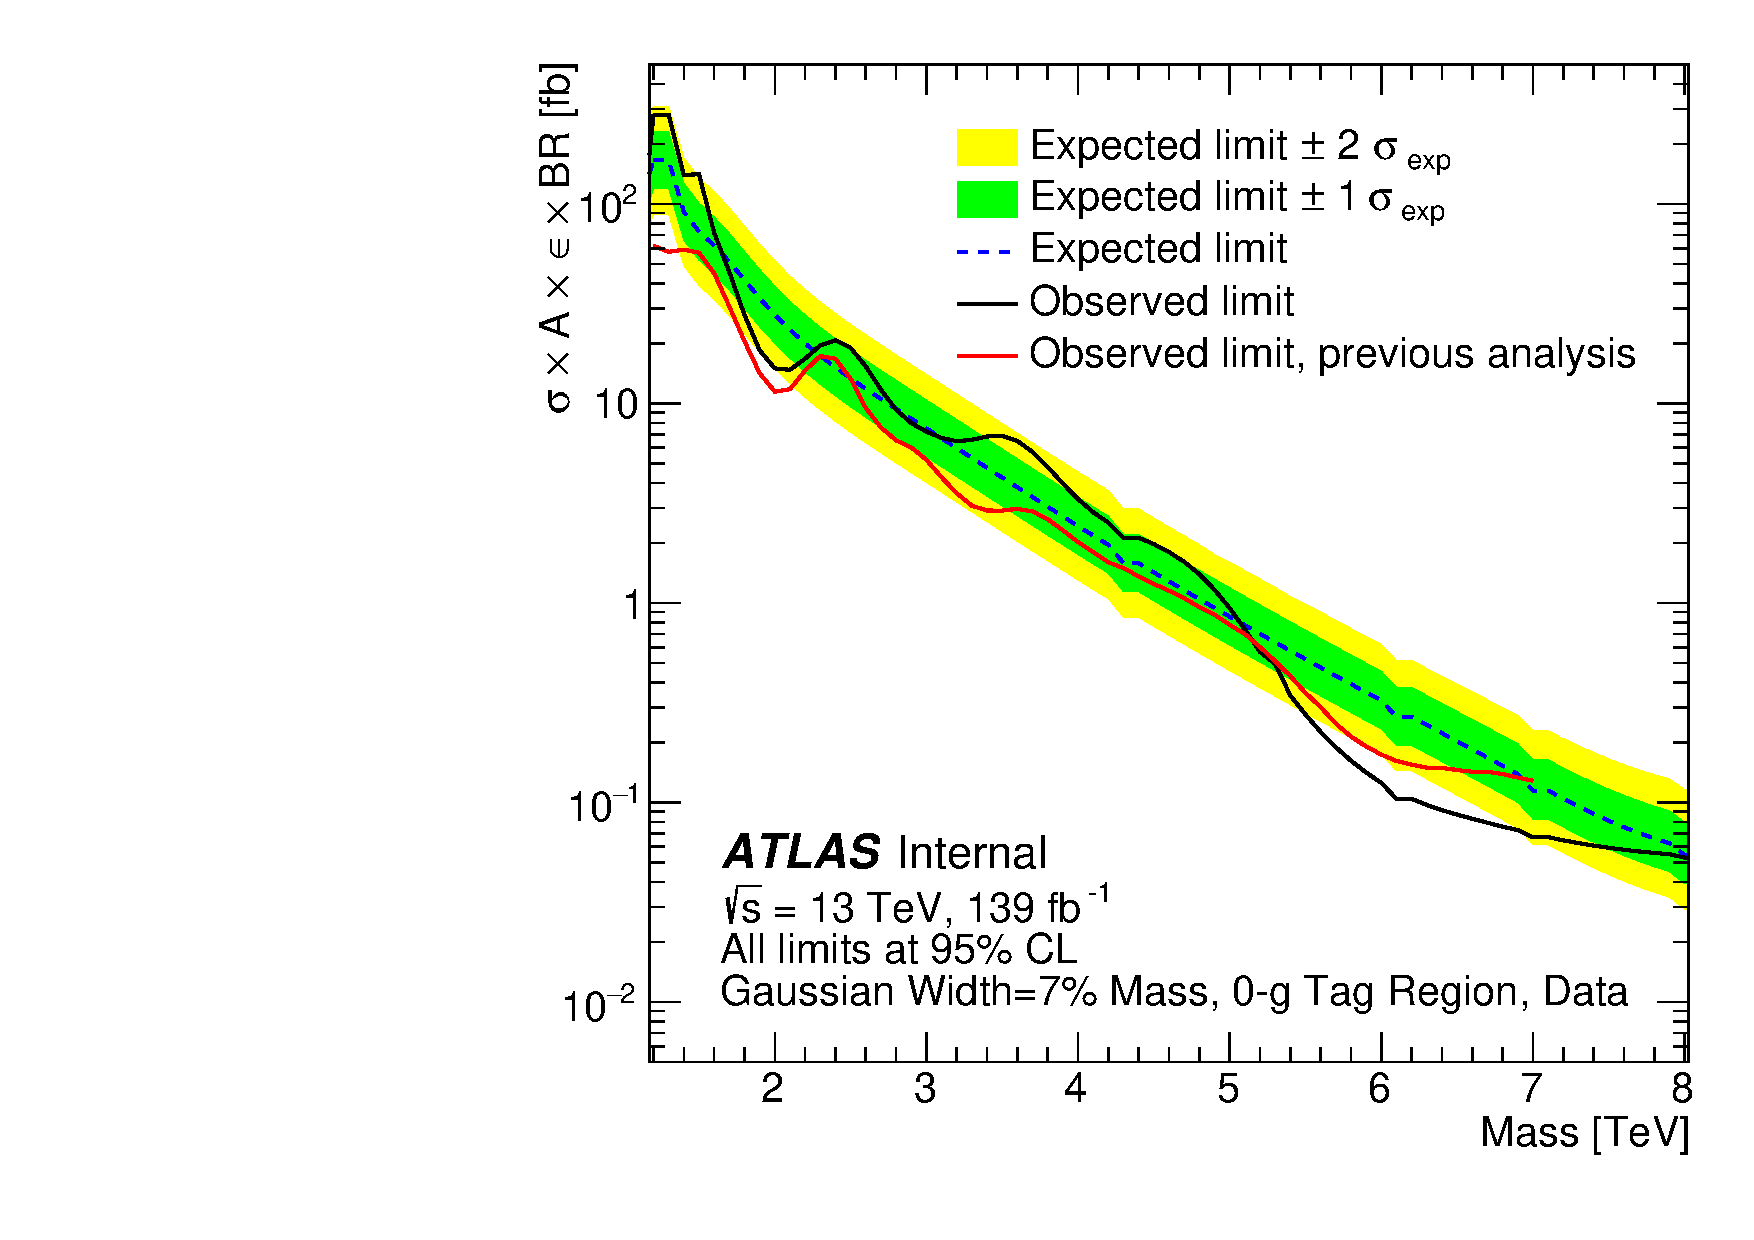
\includegraphics[width=0.4\textwidth]{fig/app-SignalIndependentLimits/Gauss_Limits_yStar0p8_Tag0_WidthPercent7_1200to8000_sigma.pdf}
            }\\
            \subfloat[10\% Width Gaussian Limits]{ 
%                \label{fig:SignalIndependentGaussianLimits_SubWidth10} % uncomment if label used. 
                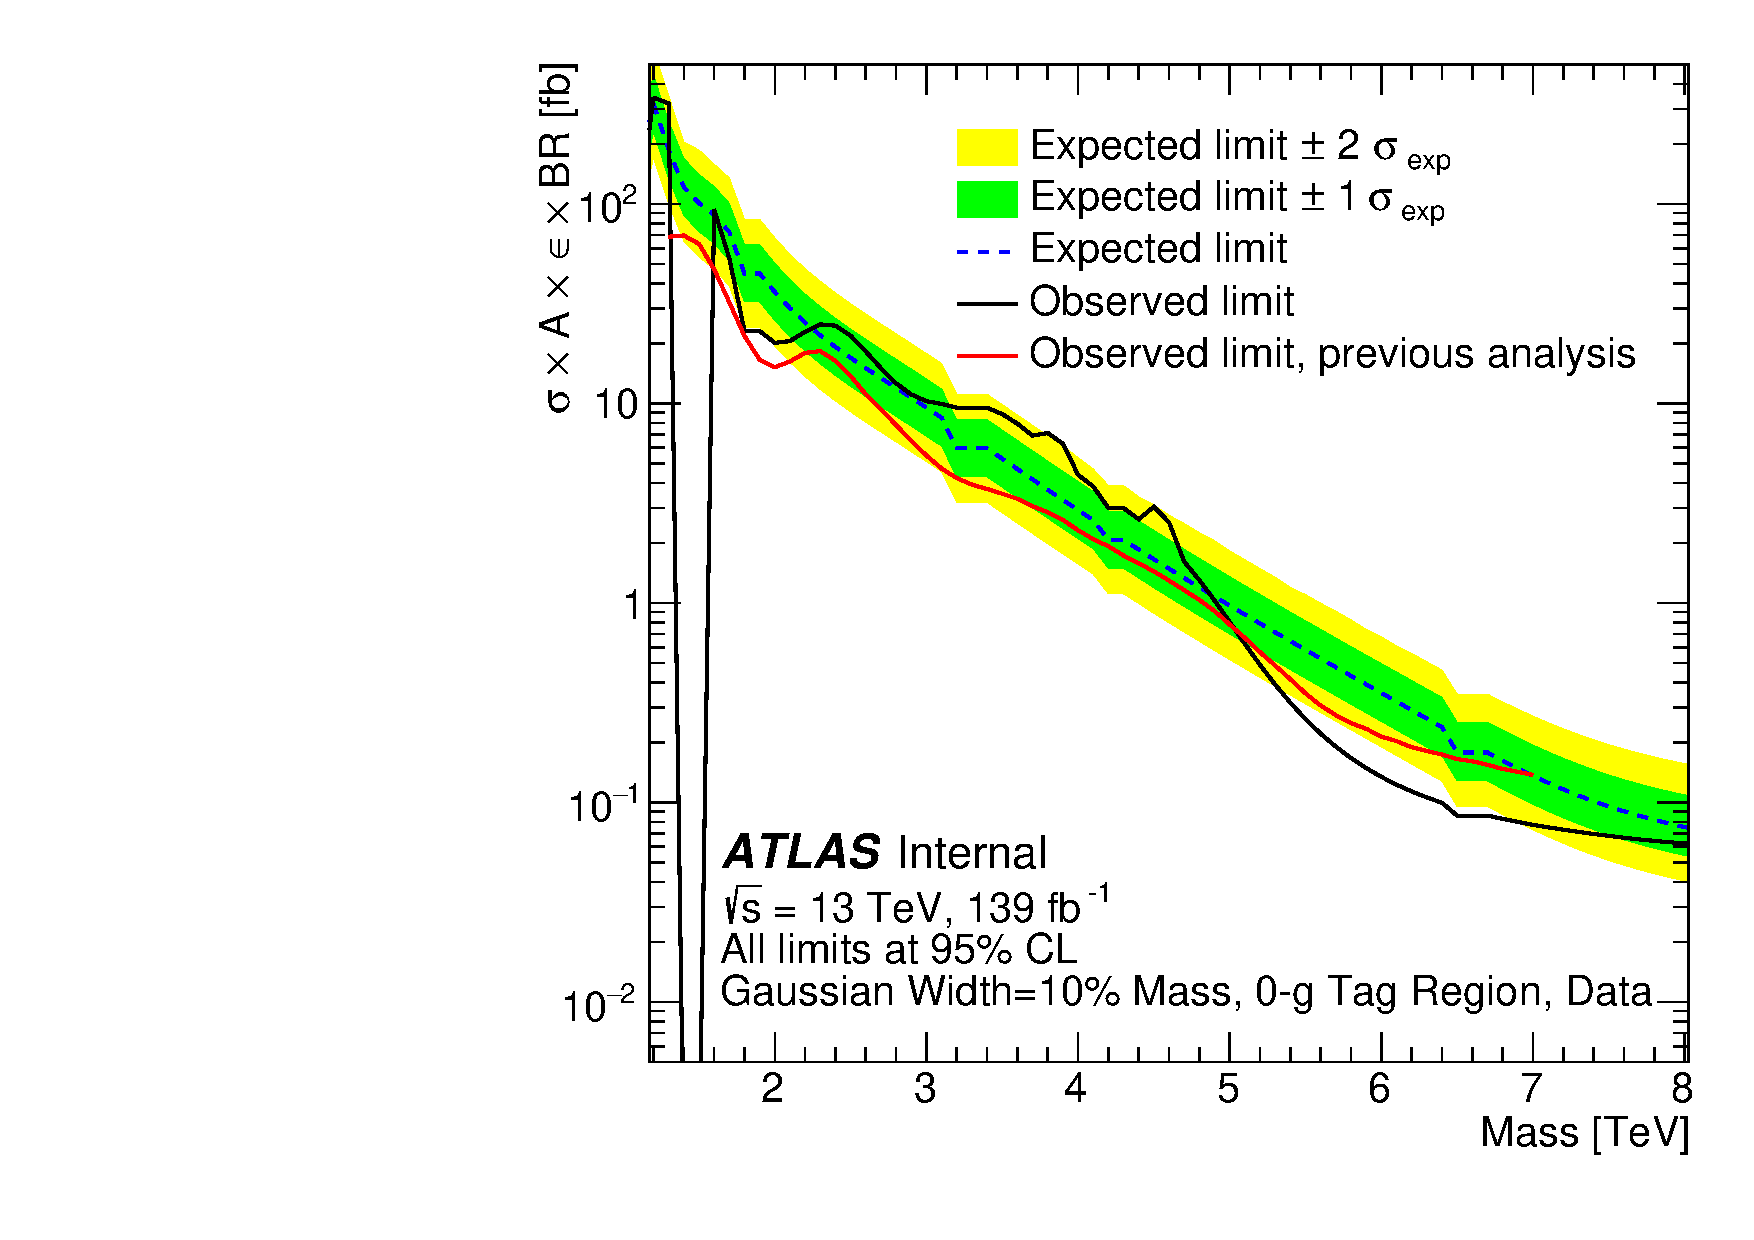
\includegraphics[width=0.4\textwidth]{fig/app-SignalIndependentLimits/Gauss_Limits_yStar0p8_Tag0_WidthPercent10_1200to8000_sigma.pdf}
            }
            \subfloat[15\% Width Gaussian Limits]{ 
%                \label{fig:SignalIndependentGaussianLimits_SubWidth15} % uncomment if label used. 
                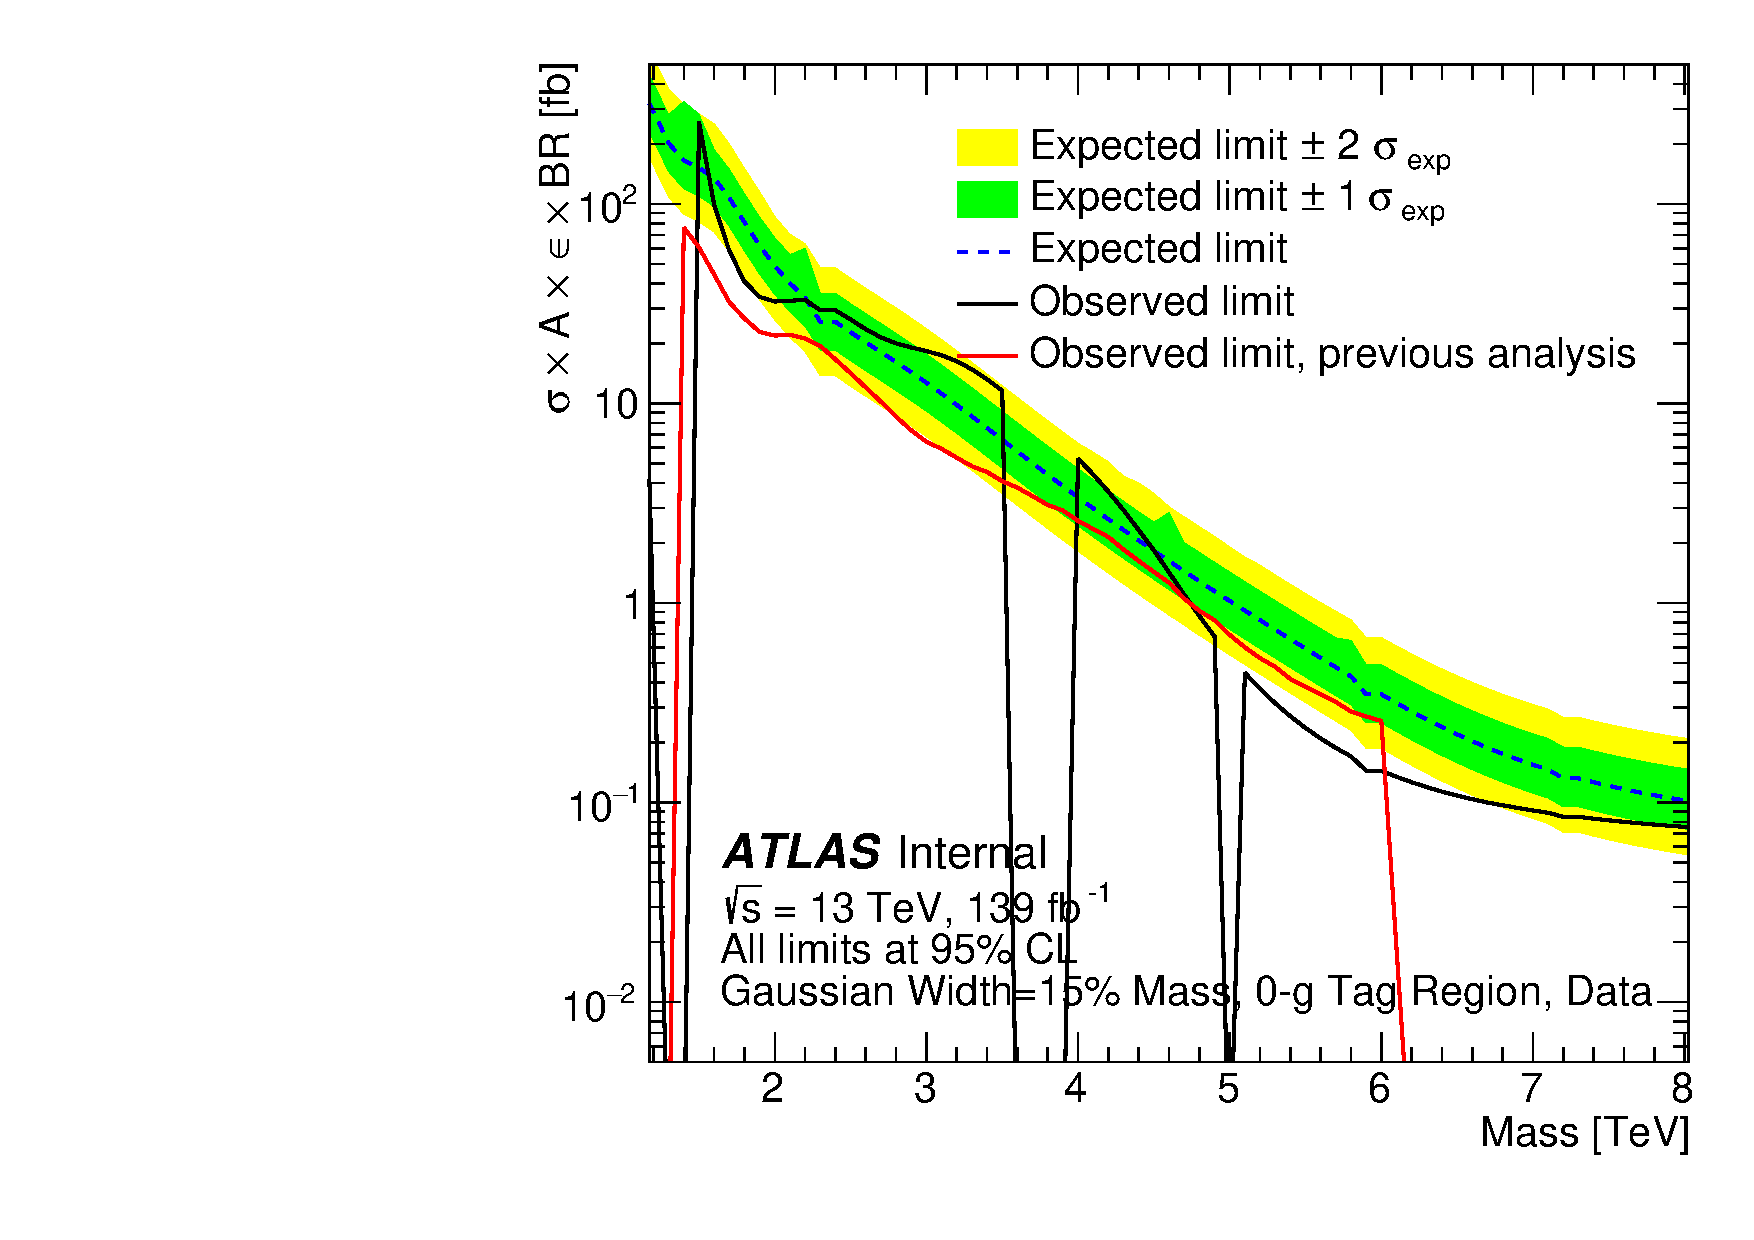
\includegraphics[width=0.4\textwidth]{fig/app-SignalIndependentLimits/Gauss_Limits_yStar0p8_Tag0_WidthPercent15_1200to8000_sigma.pdf}
            }
            \caption{Model-independent limits set in the untagged $y^{*} < 0.8$ Signal Region using Gaussian resonances of varying widths from 0\% to 15\% of their peak position without systematics included using the full 139fb$^{-1}$ Run-2 dataset.}
            \label{fig:SignalIndependentGaussianLimits_UntaggedYStar0p8}
        \end{figure}


        \begin{figure}[!htb]
            \subfloat[0\% Width Gaussian Limits]{ 
%                \label{fig:SignalIndependentGaussianLimits_SubWidth0} % uncomment if label used. 
                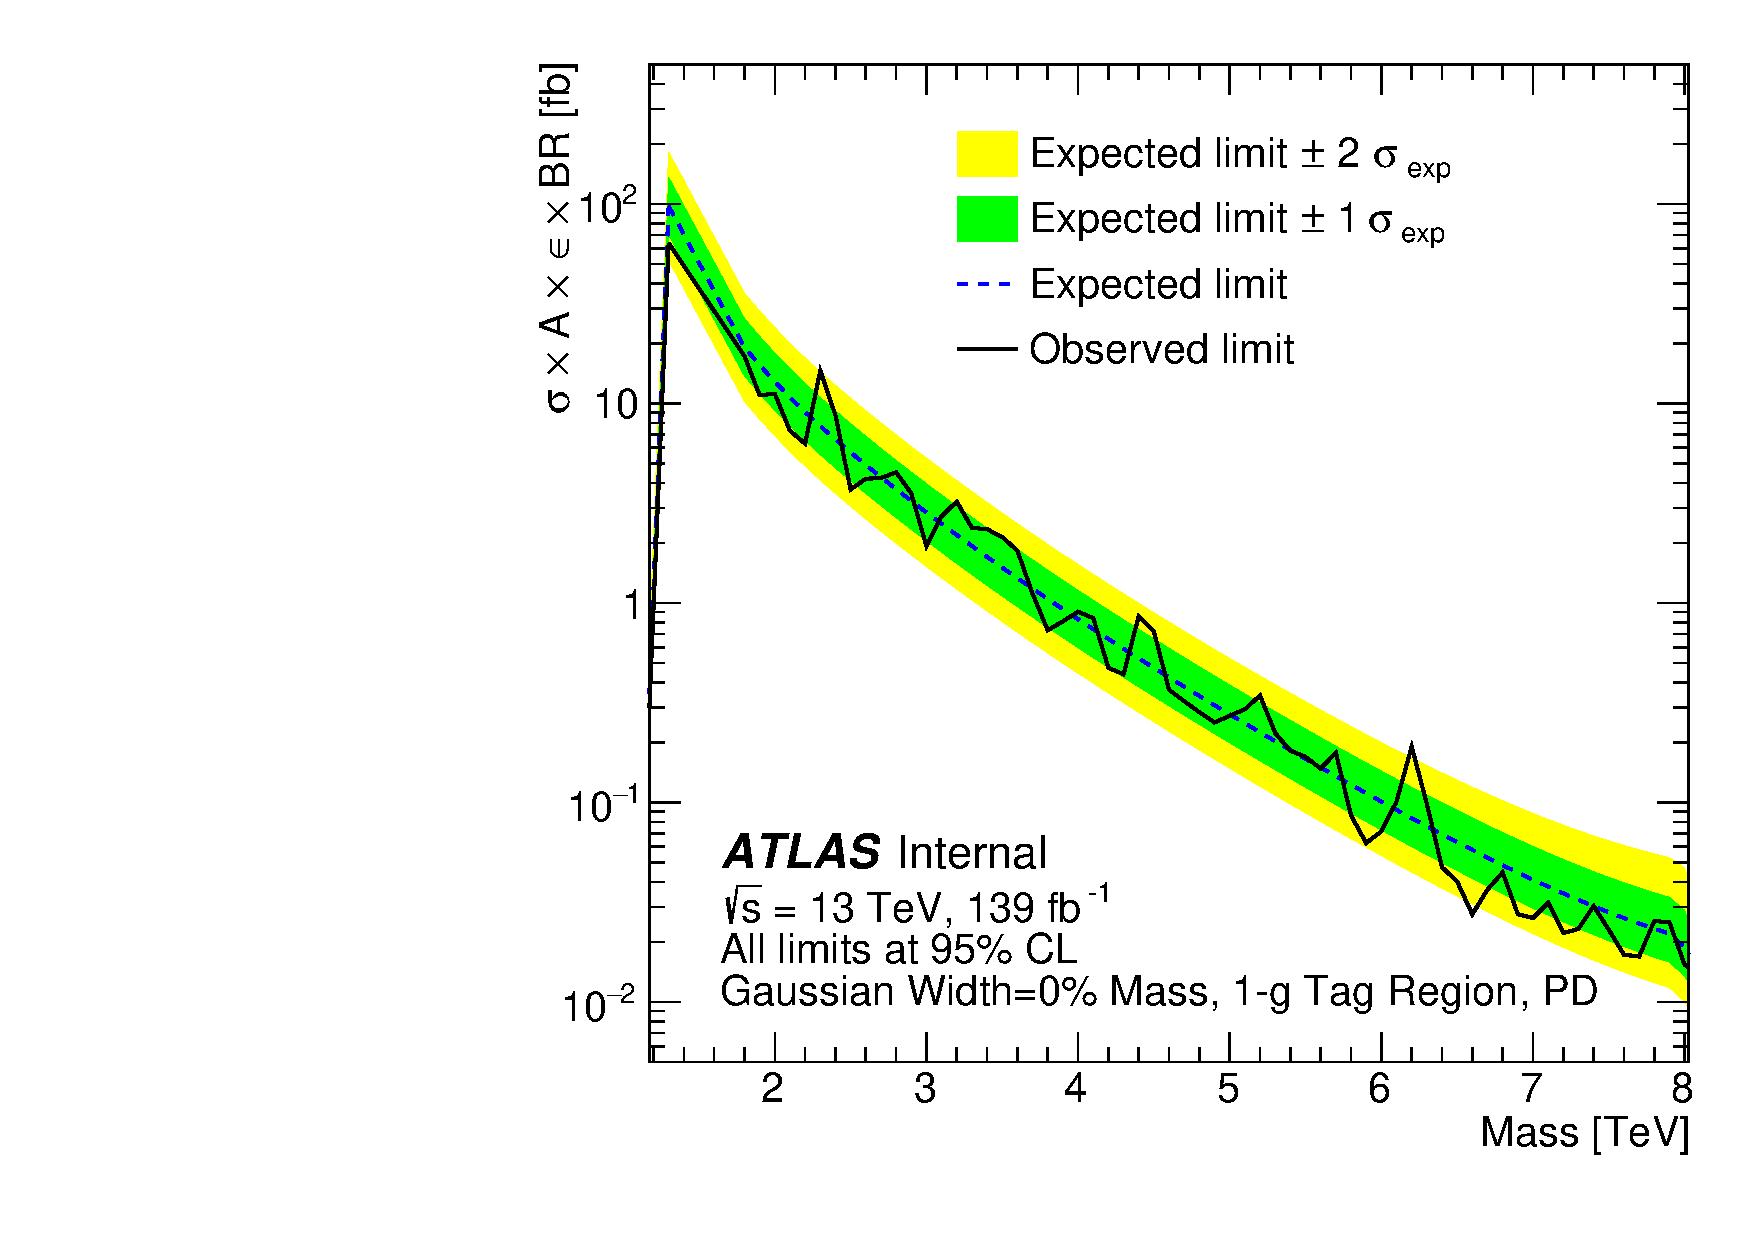
\includegraphics[width=0.4\textwidth]{fig/app-SignalIndependentLimits/Gauss_Limits_yStar0p6_Tag1_WidthPercent0_1200to8000_sigma.pdf}
            }
            \subfloat[3\% Width Gaussian Limits]{ 
%                \label{fig:SignalIndependentGaussianLimits_SubWidth3} % uncomment if label used. 
                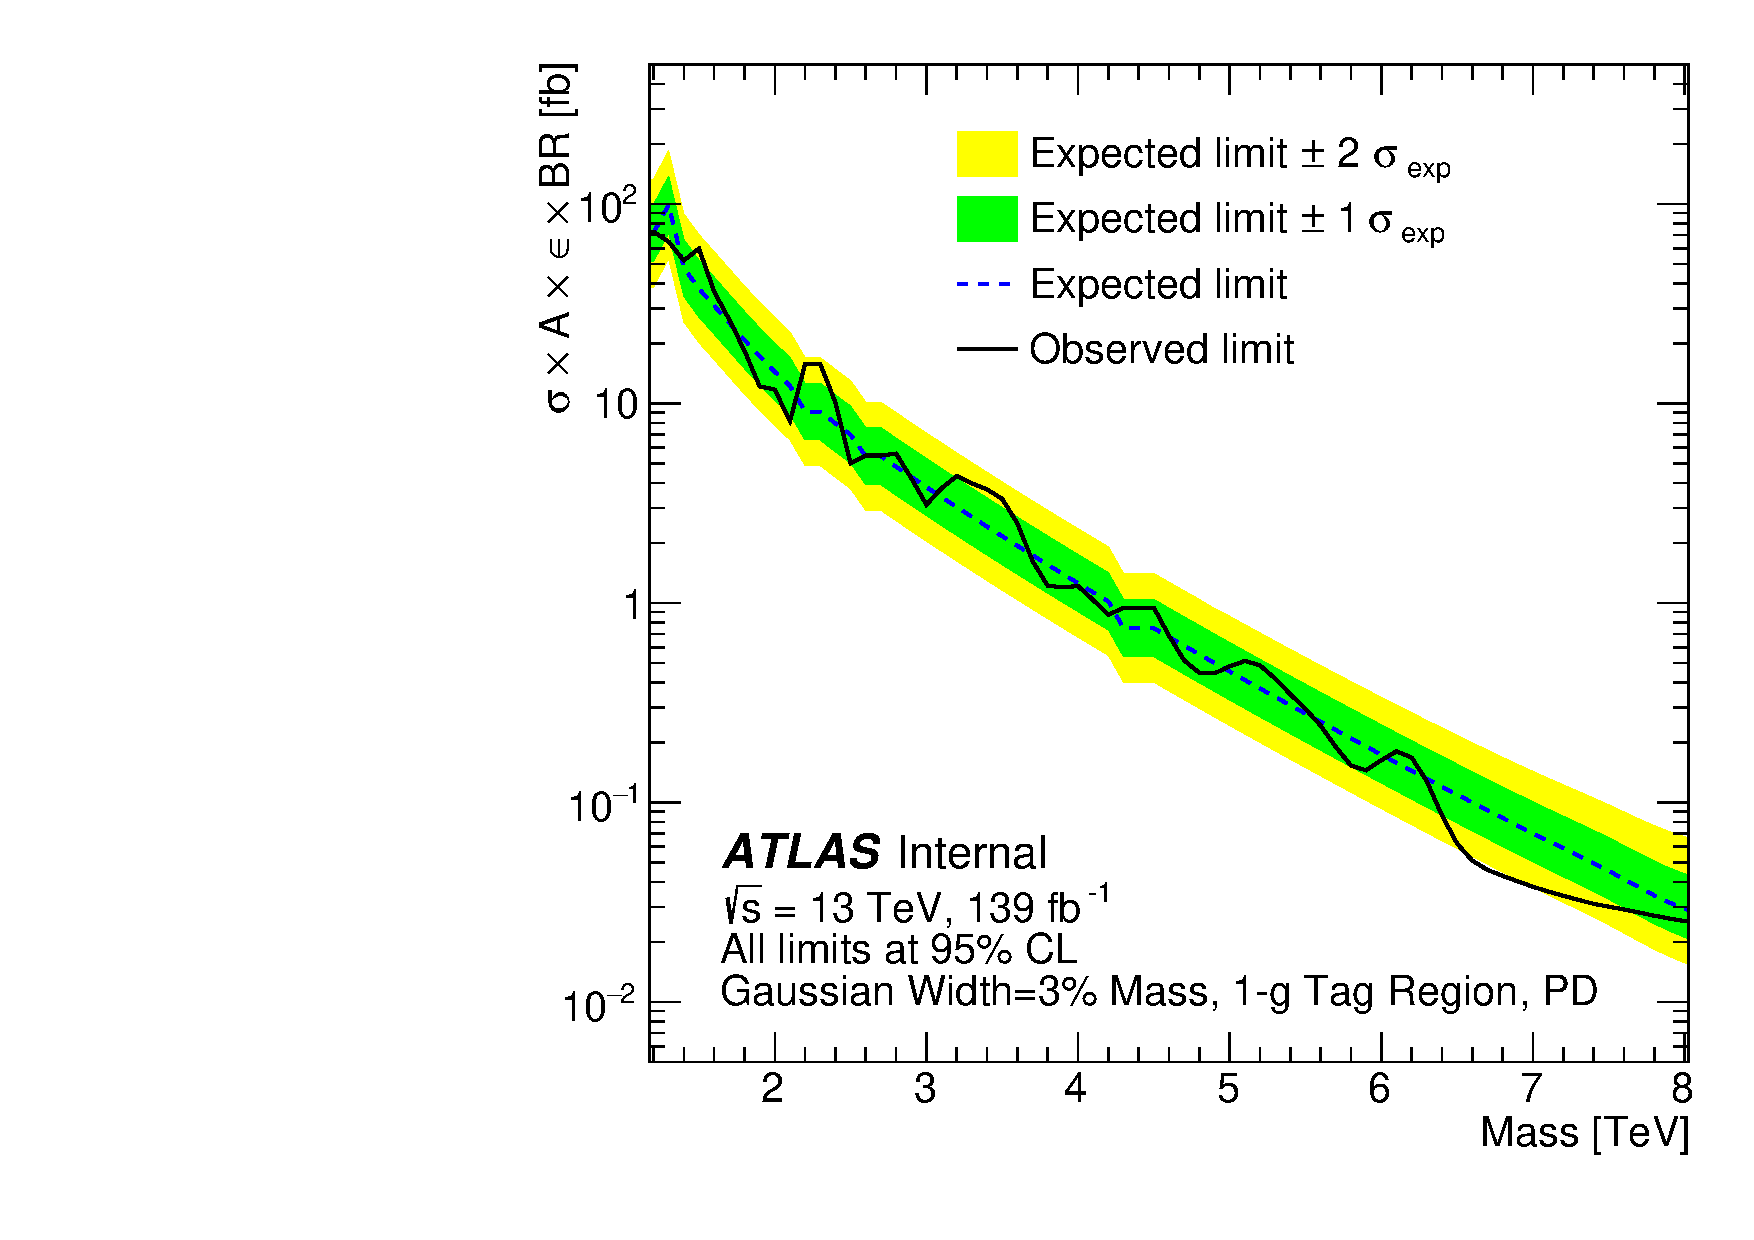
\includegraphics[width=0.4\textwidth]{fig/app-SignalIndependentLimits/Gauss_Limits_yStar0p6_Tag1_WidthPercent3_1200to8000_sigma.pdf}
            }\\
            \subfloat[5\% Width Gaussian Limits]{ 
%                \label{fig:SignalIndependentGaussianLimits_SubWidth5} % uncomment if label used. 
                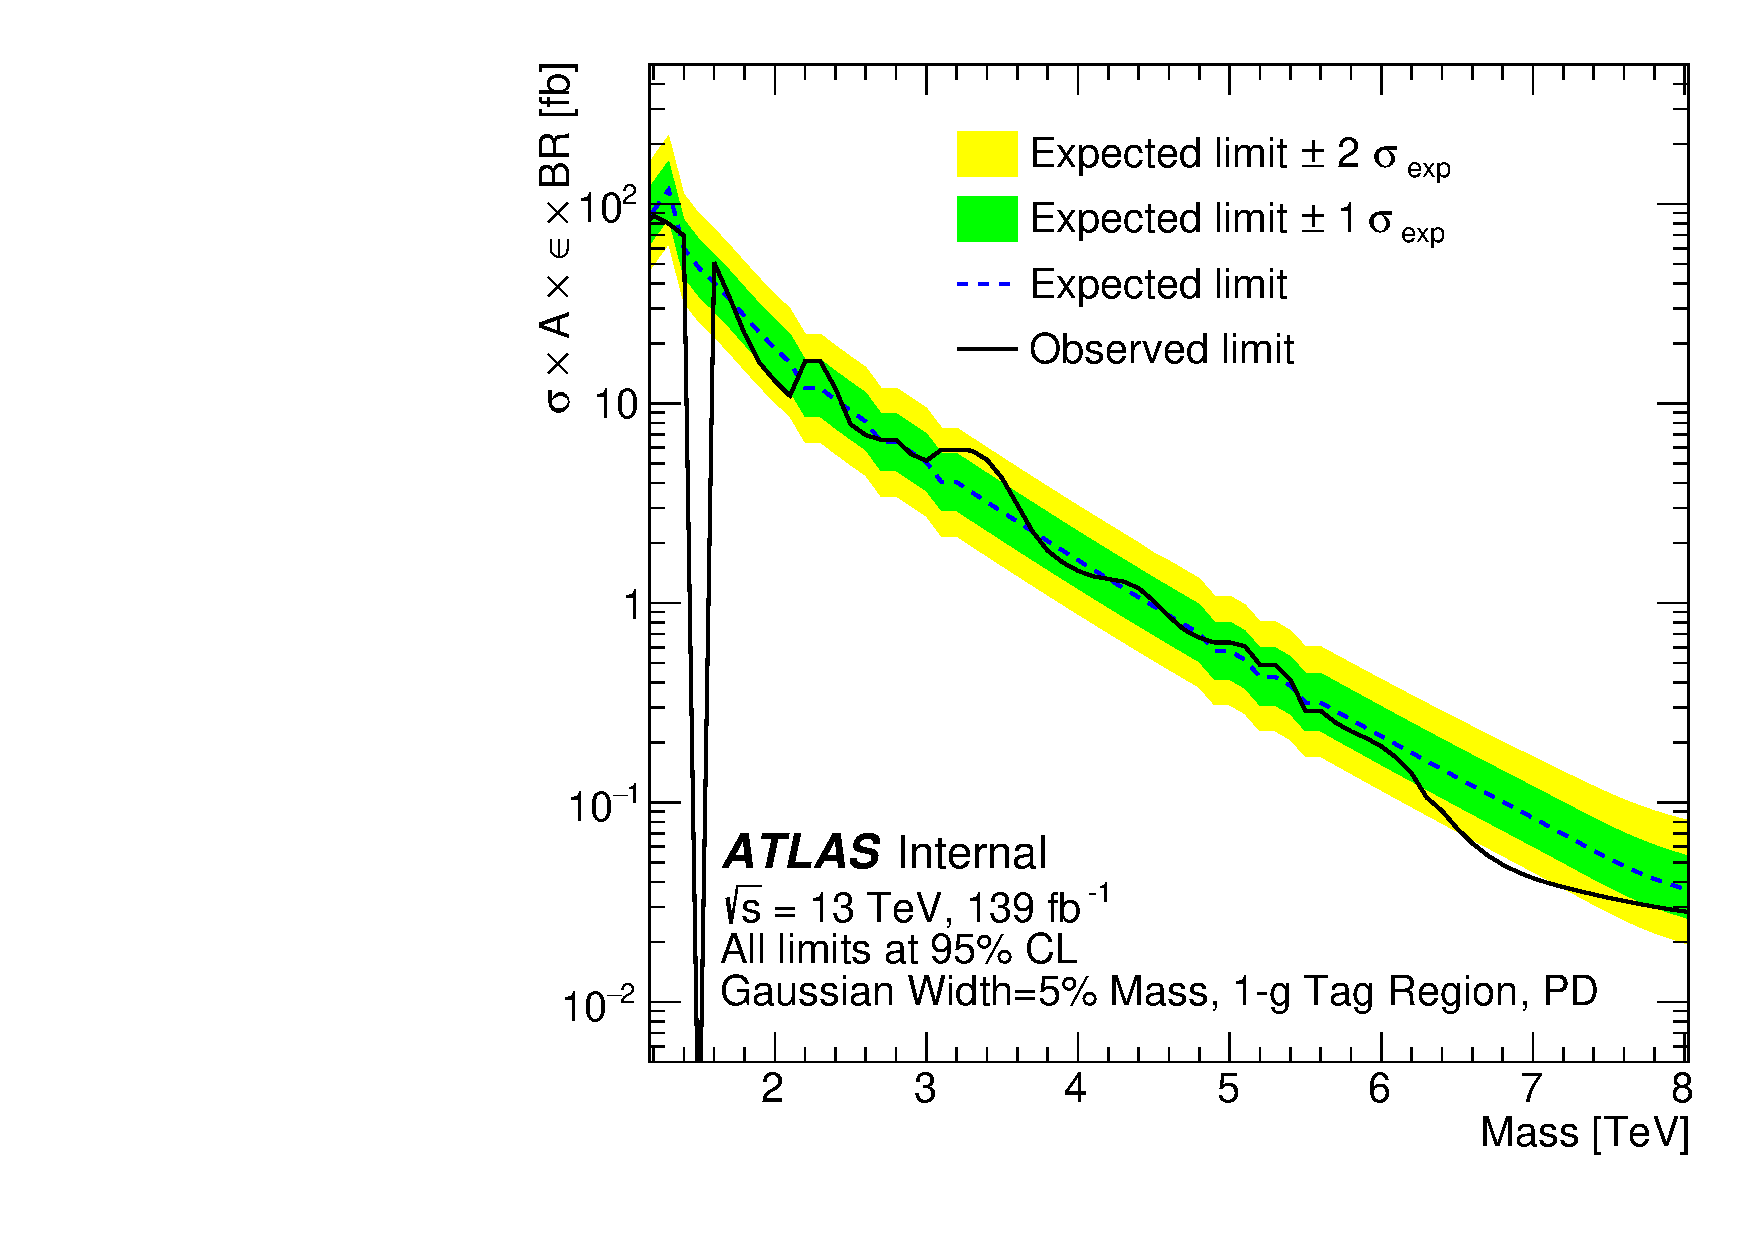
\includegraphics[width=0.4\textwidth]{fig/app-SignalIndependentLimits/Gauss_Limits_yStar0p6_Tag1_WidthPercent5_1200to8000_sigma.pdf}
            }
            \subfloat[7\% Width Gaussian Limits]{ 
%                \label{fig:SignalIndependentGaussianLimits_SubWidth7} % uncomment if label used. 
                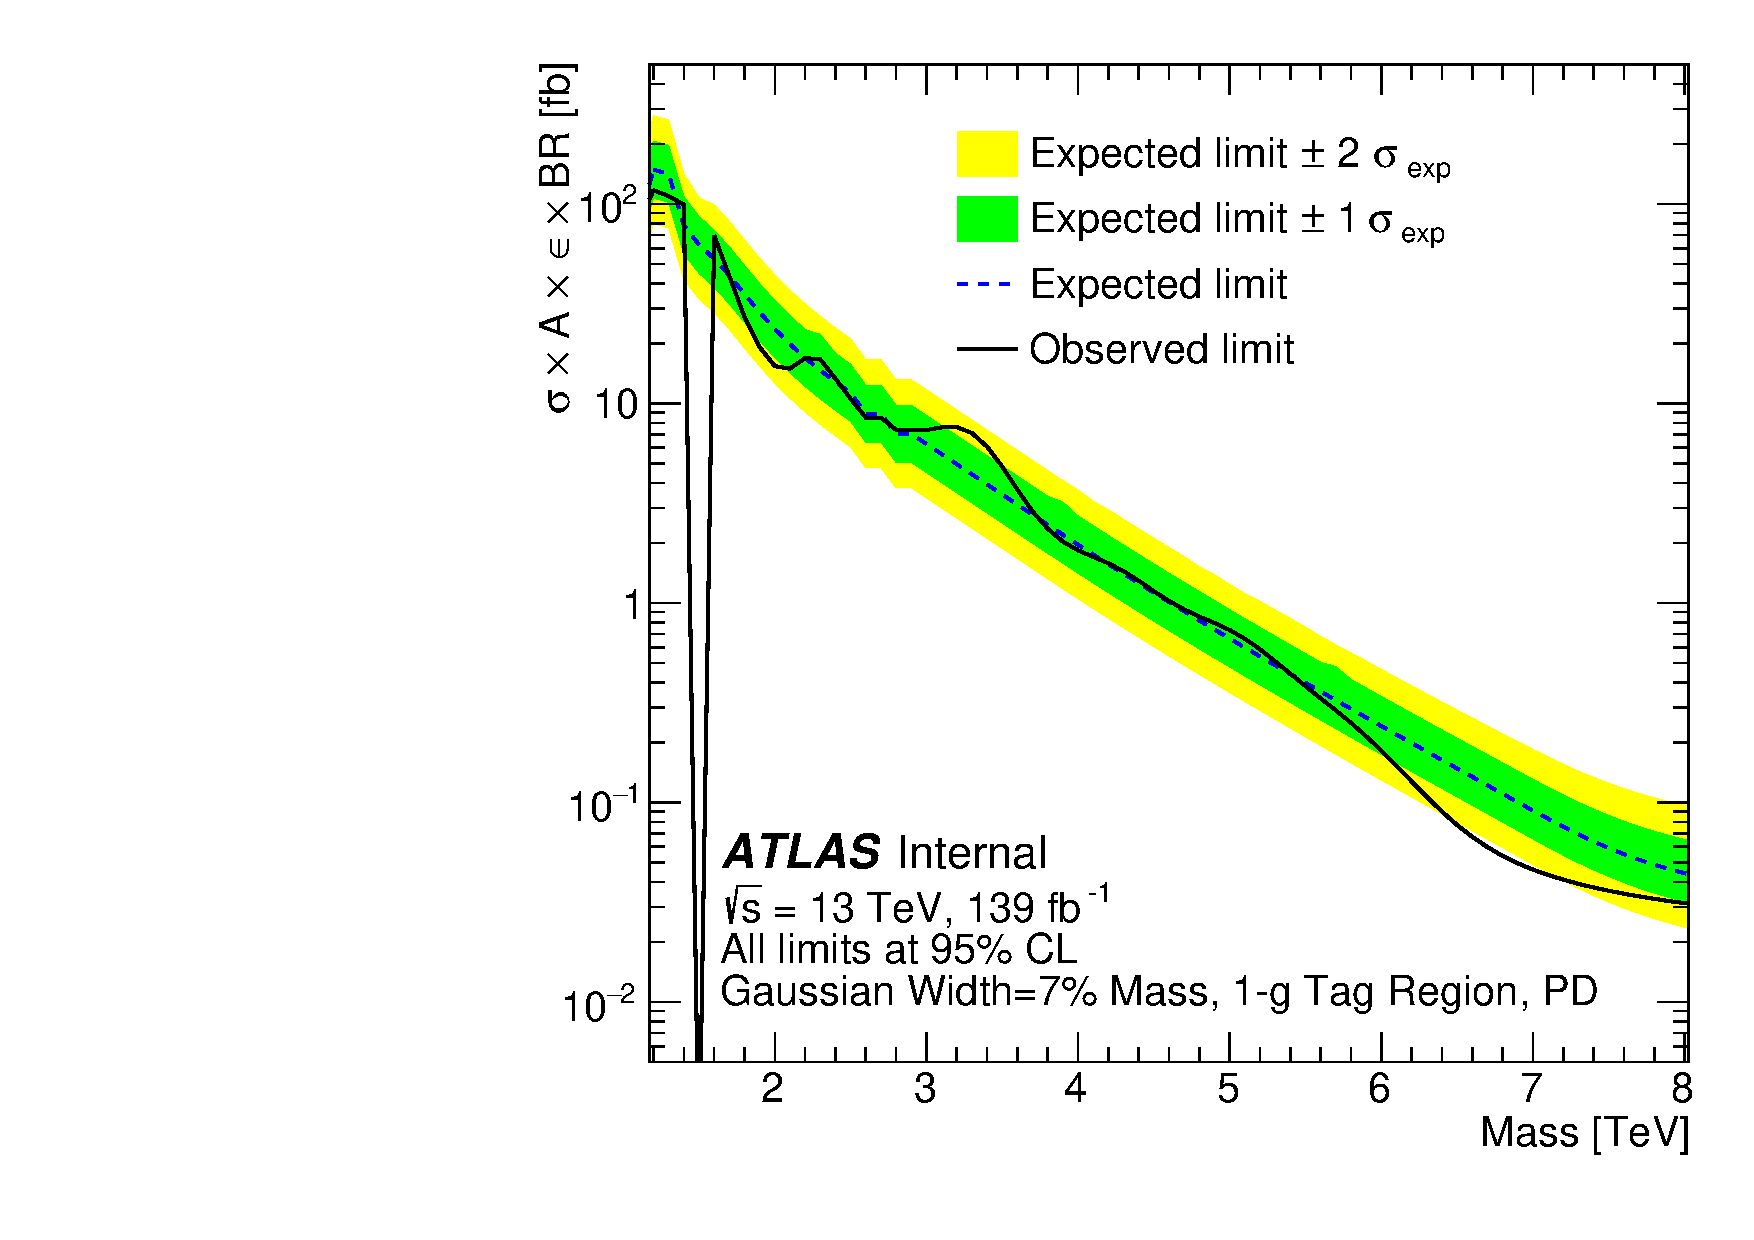
\includegraphics[width=0.4\textwidth]{fig/app-SignalIndependentLimits/Gauss_Limits_yStar0p6_Tag1_WidthPercent7_1200to8000_sigma.pdf}
            }\\
            \subfloat[10\% Width Gaussian Limits]{ 
%                \label{fig:SignalIndependentGaussianLimits_SubWidth10} % uncomment if label used. 
                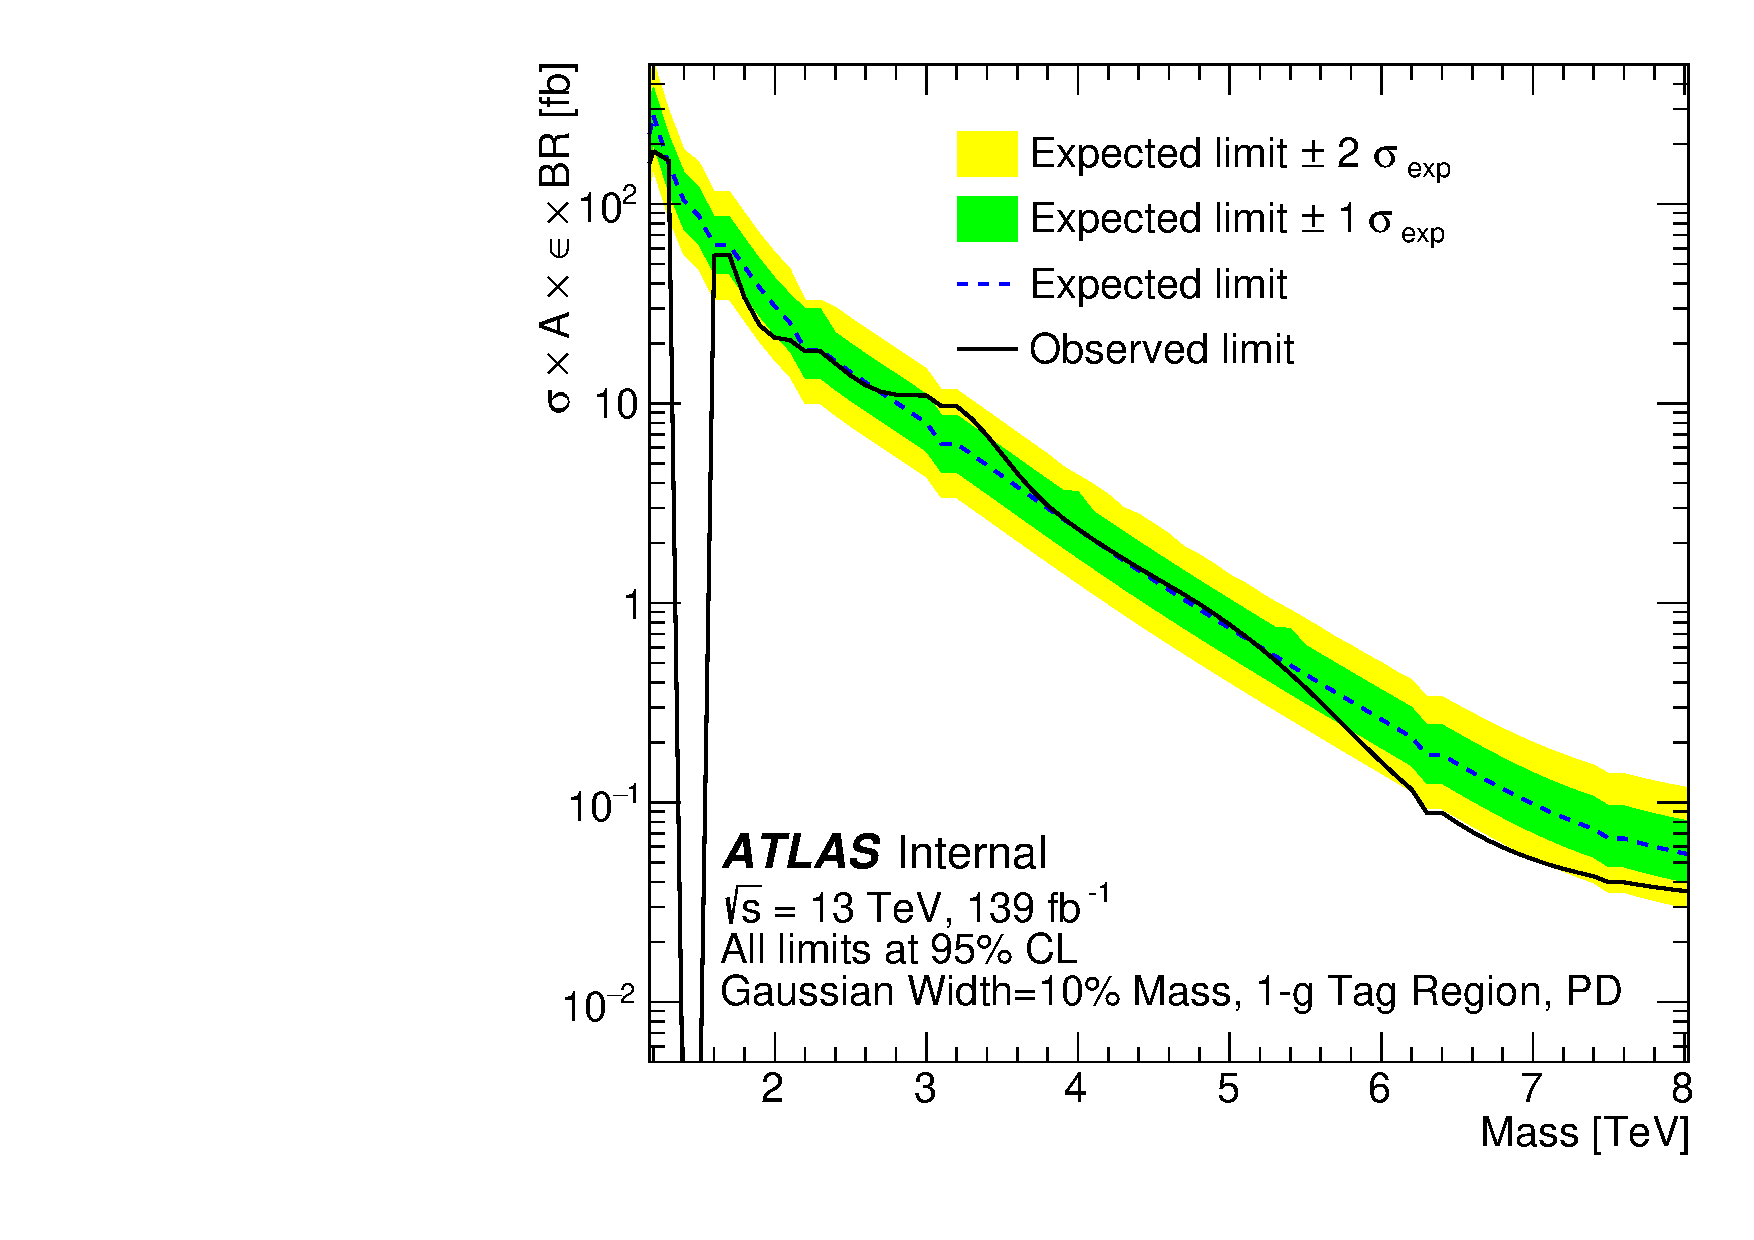
\includegraphics[width=0.4\textwidth]{fig/app-SignalIndependentLimits/Gauss_Limits_yStar0p6_Tag1_WidthPercent10_1200to8000_sigma.pdf}
            }
            \subfloat[15\% Width Gaussian Limits]{ 
%                \label{fig:SignalIndependentGaussianLimits_SubWidth15} % uncomment if label used. 
                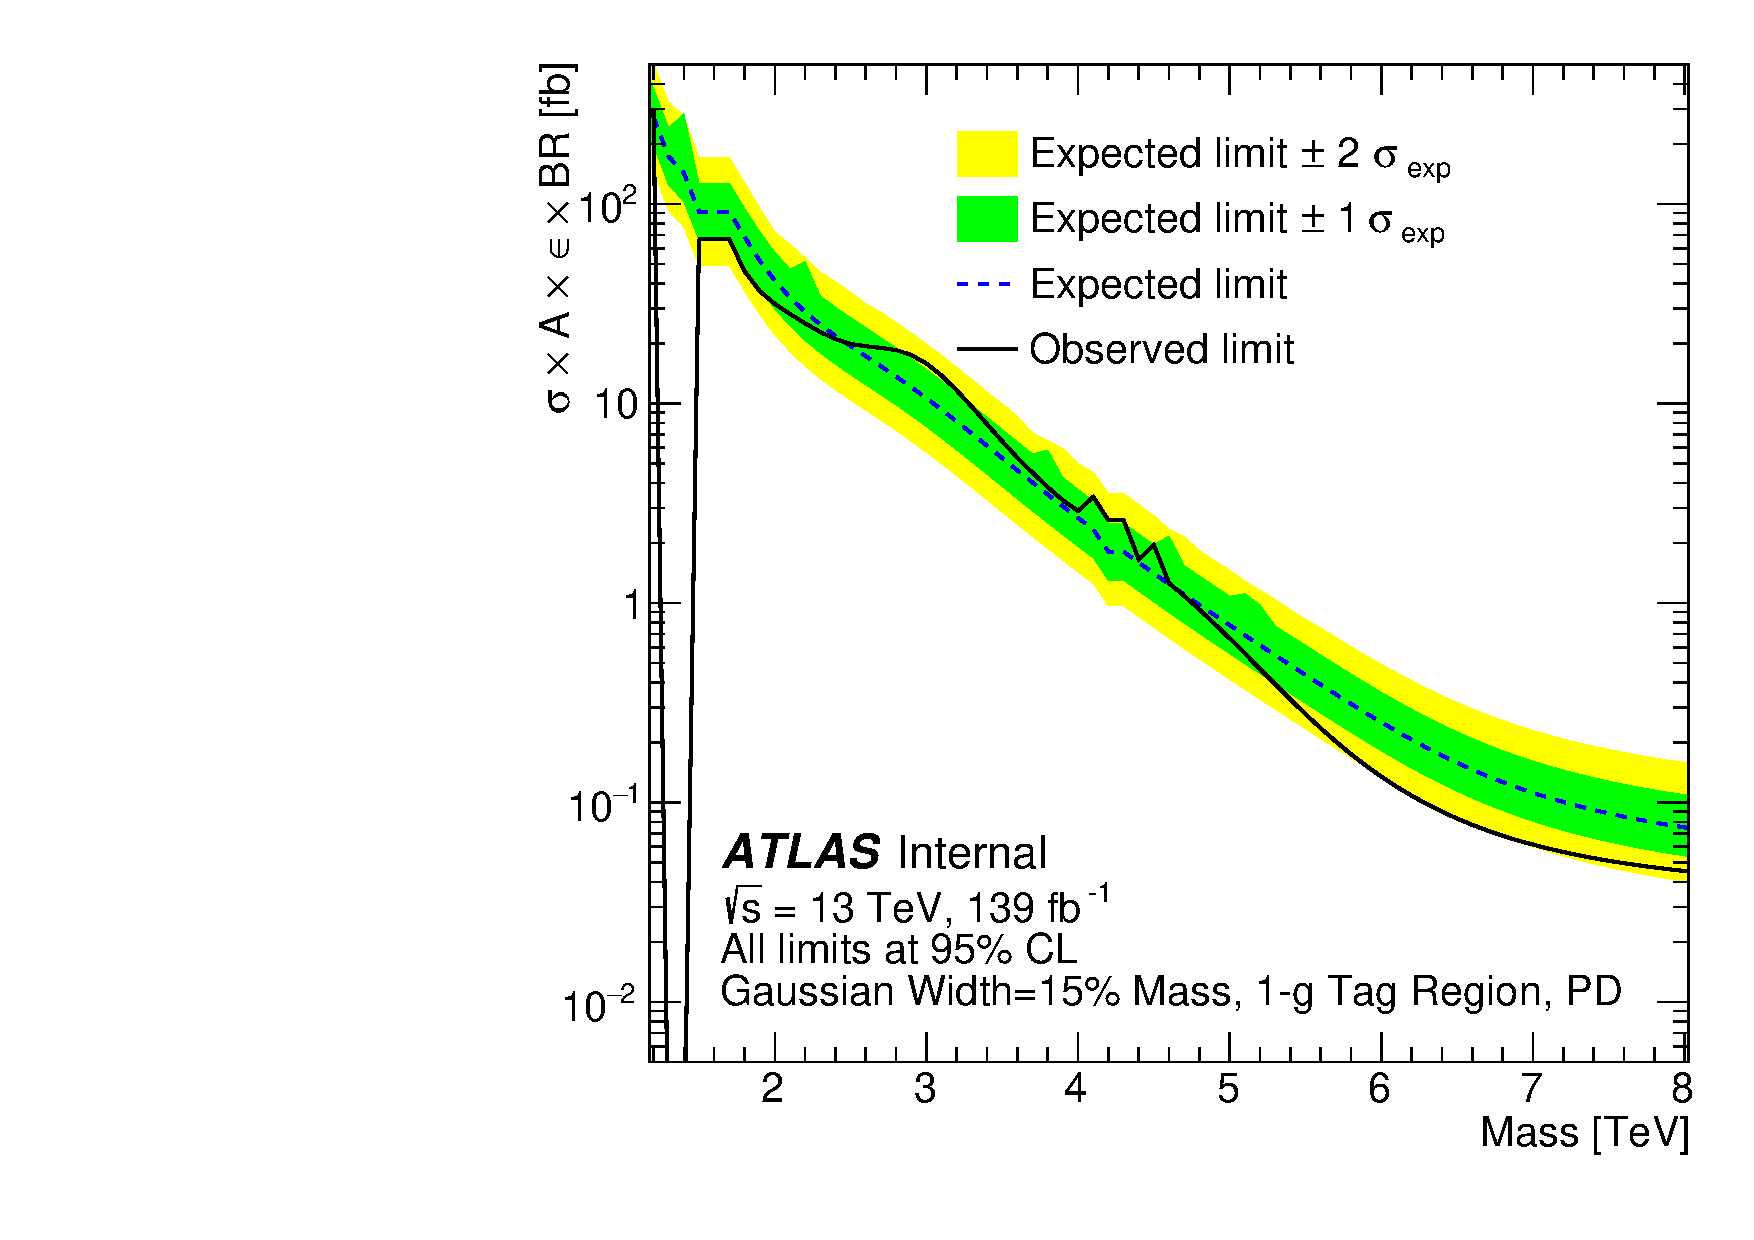
\includegraphics[width=0.4\textwidth]{fig/app-SignalIndependentLimits/Gauss_Limits_yStar0p6_Tag1_WidthPercent15_1200to8000_sigma.pdf}
            }
            \caption{Model-independent limits set in the 1-$g$ tagged $y^{*} < 0.6$ Signal Region using Gaussian resonances of varying widths from 0\% to 15\% of their peak position without systematics included using the full 139fb$^{-1}$ Run-2 dataset.}
            \label{fig:SignalIndependentGaussianLimits_1gYStar0p6}
        \end{figure}

        \begin{figure}[!htb]
            \subfloat[0\% Width Gaussian Limits]{ 
%                \label{fig:SignalIndependentGaussianLimits_SubWidth0} % uncomment if label used. 
                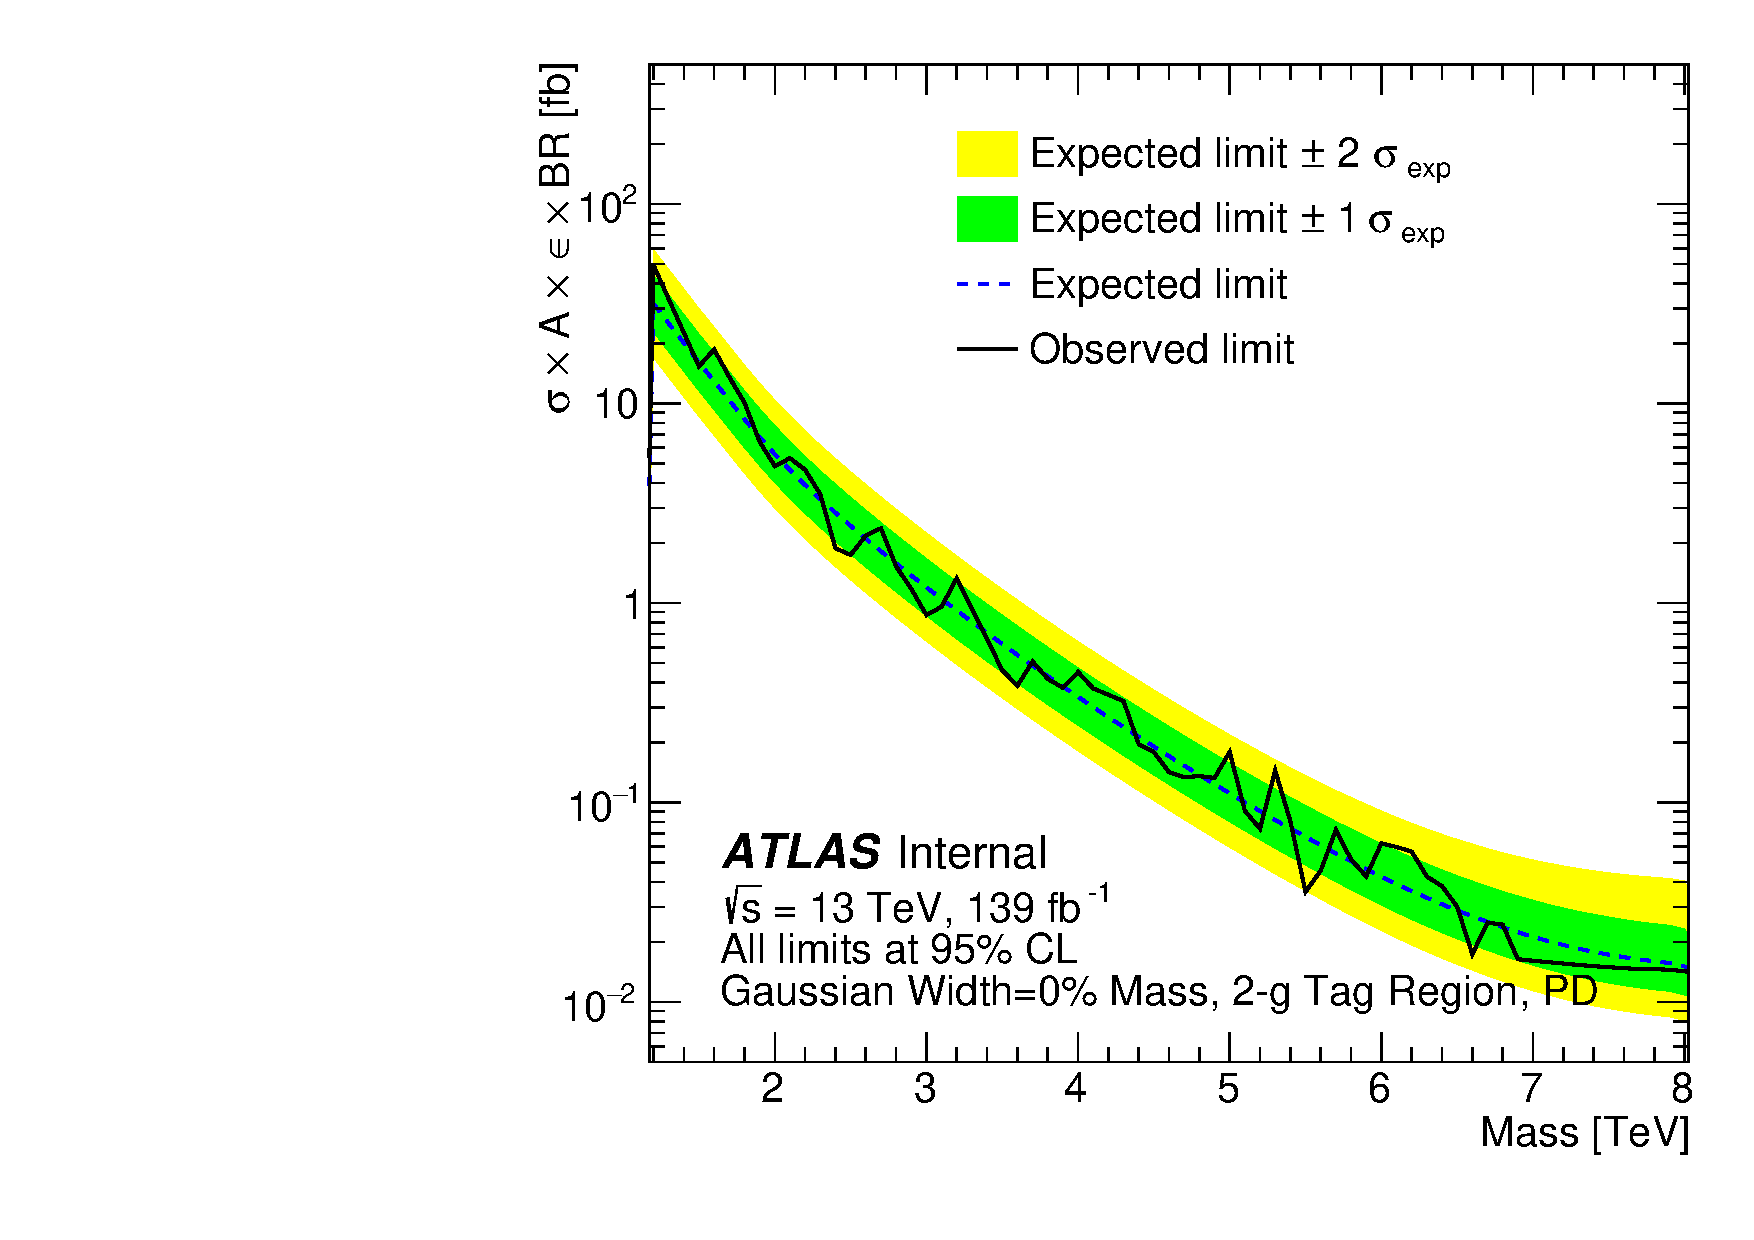
\includegraphics[width=0.4\textwidth]{fig/app-SignalIndependentLimits/Gauss_Limits_yStar0p8_Tag2_WidthPercent0_1200to8000_sigma.pdf}
            }
            \subfloat[3\% Width Gaussian Limits]{ 
%                \label{fig:SignalIndependentGaussianLimits_SubWidth3} % uncomment if label used. 
                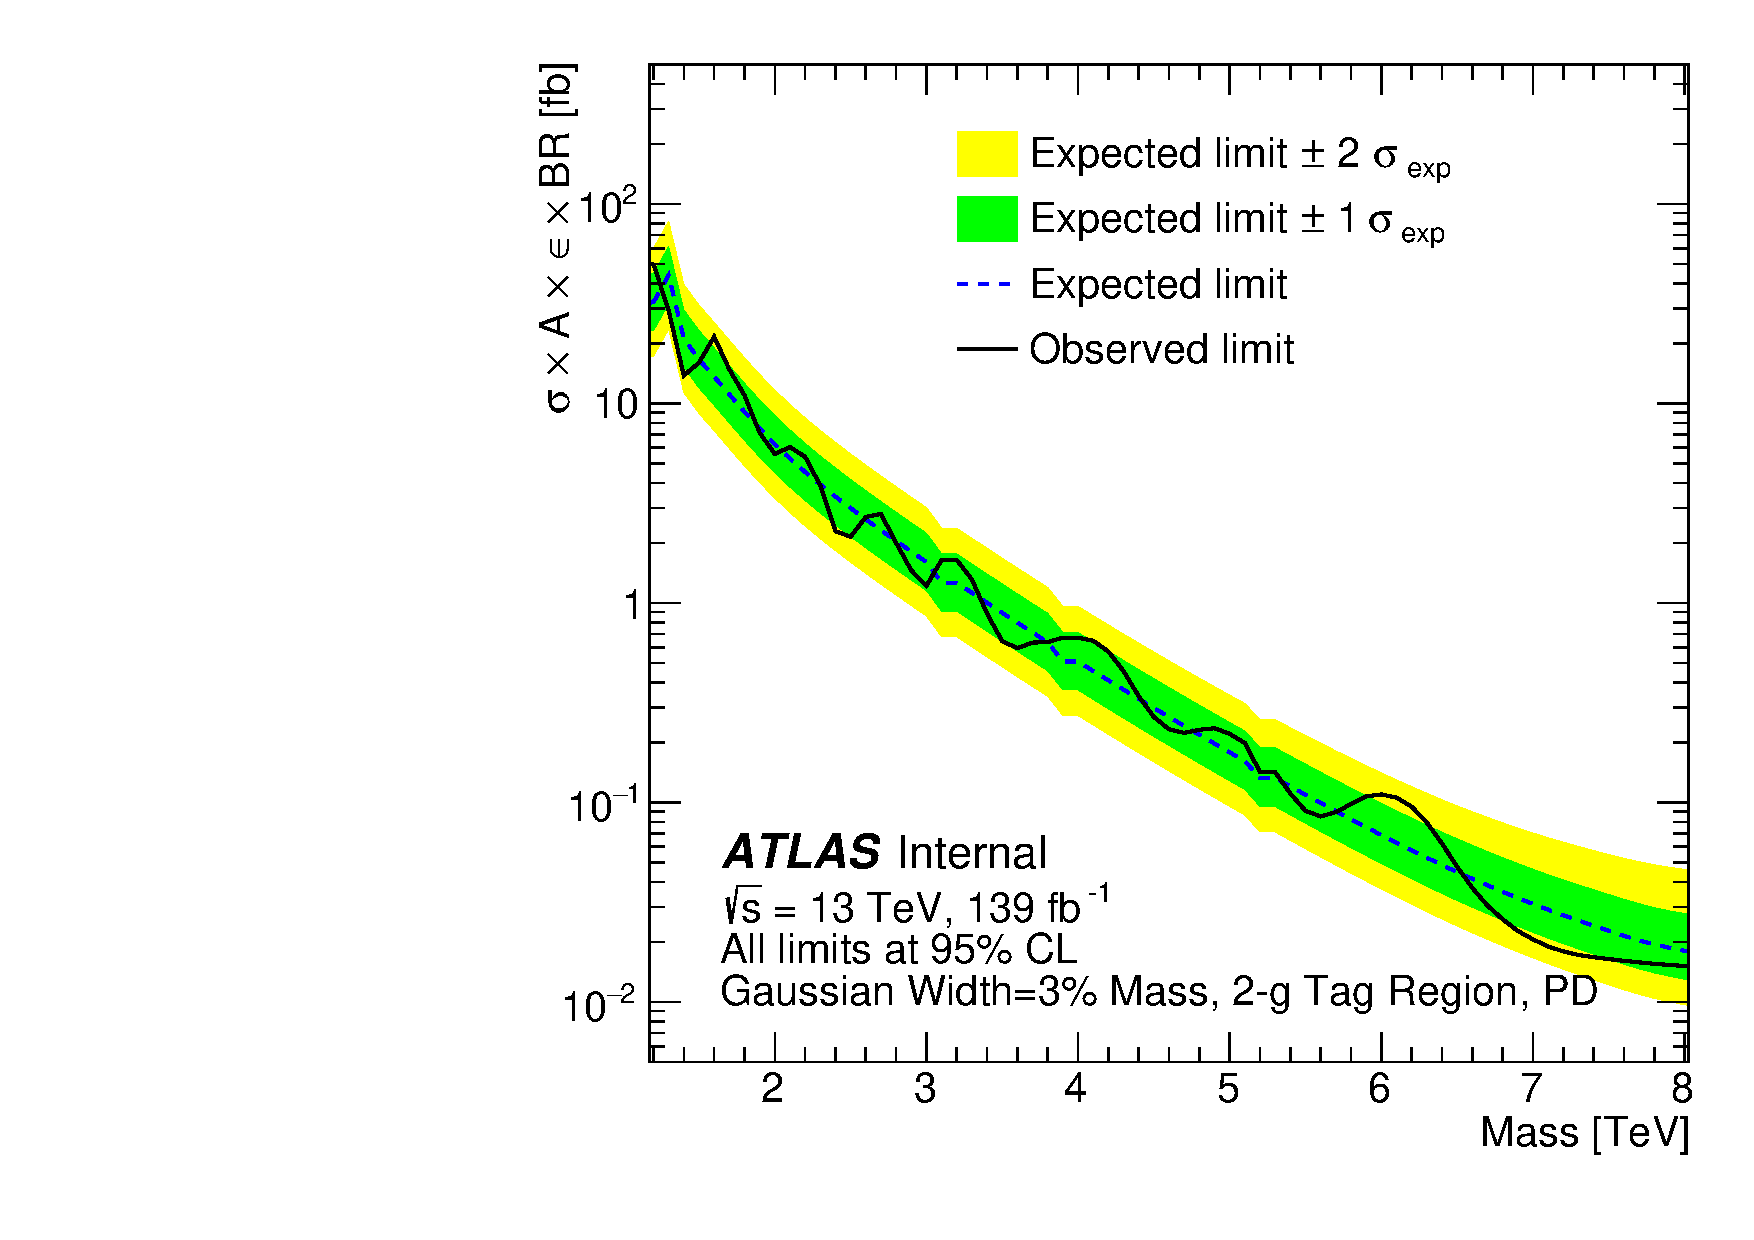
\includegraphics[width=0.4\textwidth]{fig/app-SignalIndependentLimits/Gauss_Limits_yStar0p8_Tag2_WidthPercent3_1200to8000_sigma.pdf}
            }\\
            \subfloat[5\% Width Gaussian Limits]{ 
%                \label{fig:SignalIndependentGaussianLimits_SubWidth5} % uncomment if label used. 
                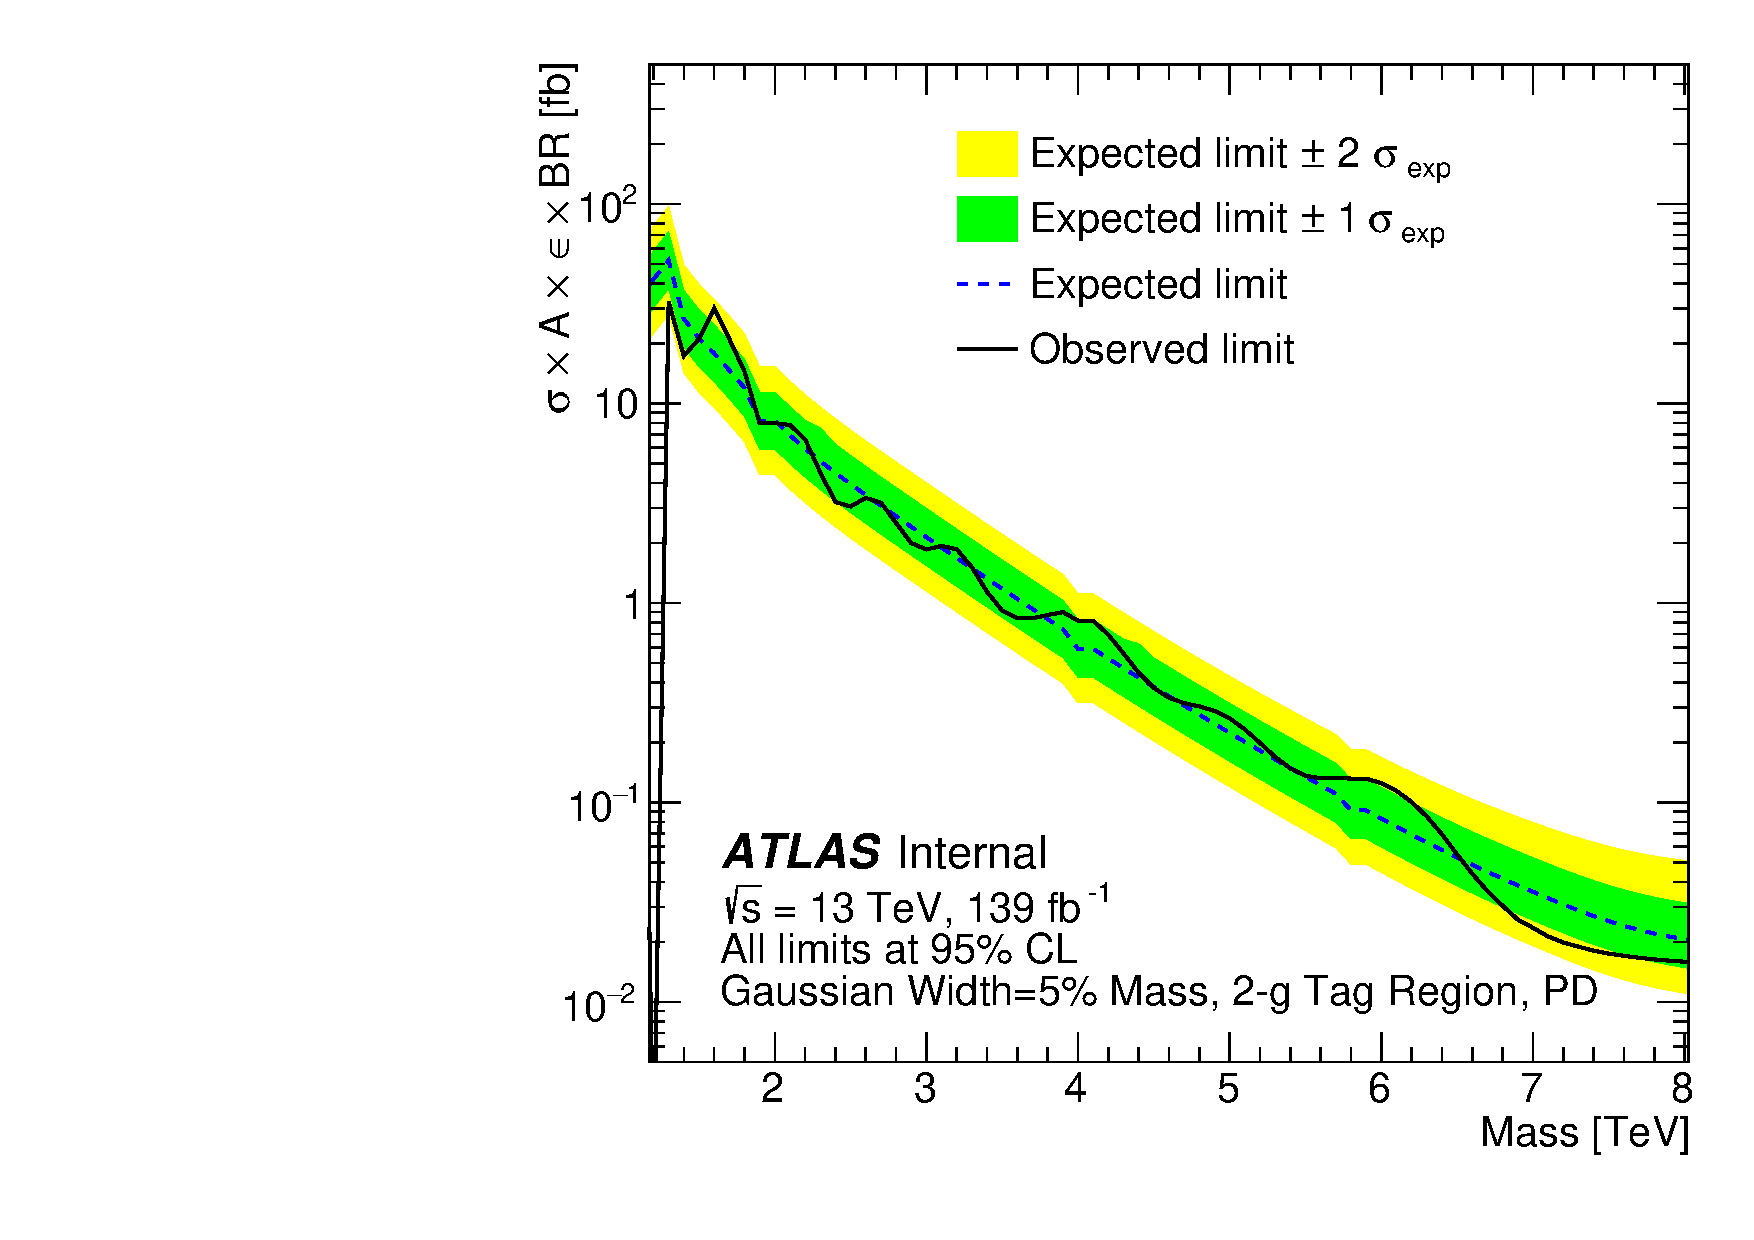
\includegraphics[width=0.4\textwidth]{fig/app-SignalIndependentLimits/Gauss_Limits_yStar0p8_Tag2_WidthPercent5_1200to8000_sigma.pdf}
            }
            \subfloat[7\% Width Gaussian Limits]{ 
%                \label{fig:SignalIndependentGaussianLimits_SubWidth7} % uncomment if label used. 
                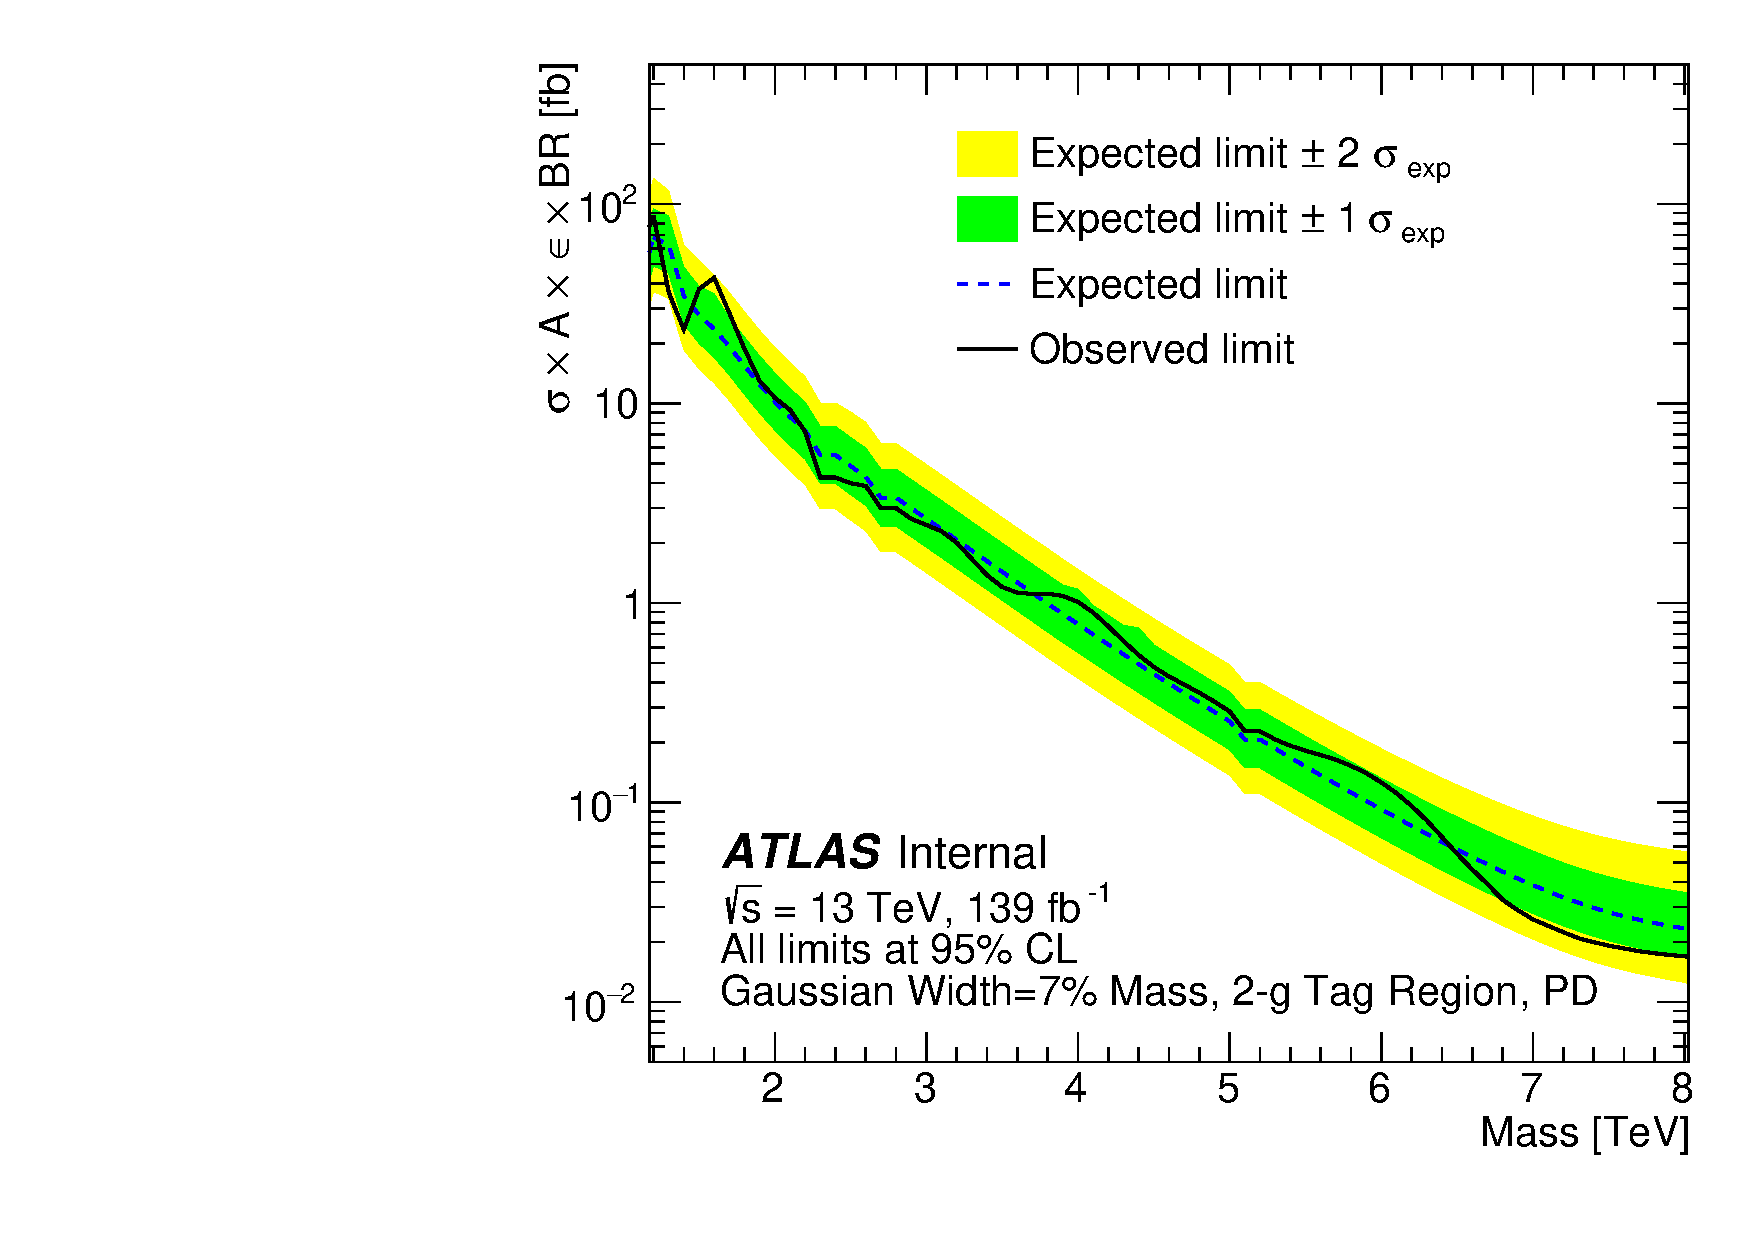
\includegraphics[width=0.4\textwidth]{fig/app-SignalIndependentLimits/Gauss_Limits_yStar0p8_Tag2_WidthPercent7_1200to8000_sigma.pdf}
            }\\
            \subfloat[10\% Width Gaussian Limits]{ 
%                \label{fig:SignalIndependentGaussianLimits_SubWidth10} % uncomment if label used. 
                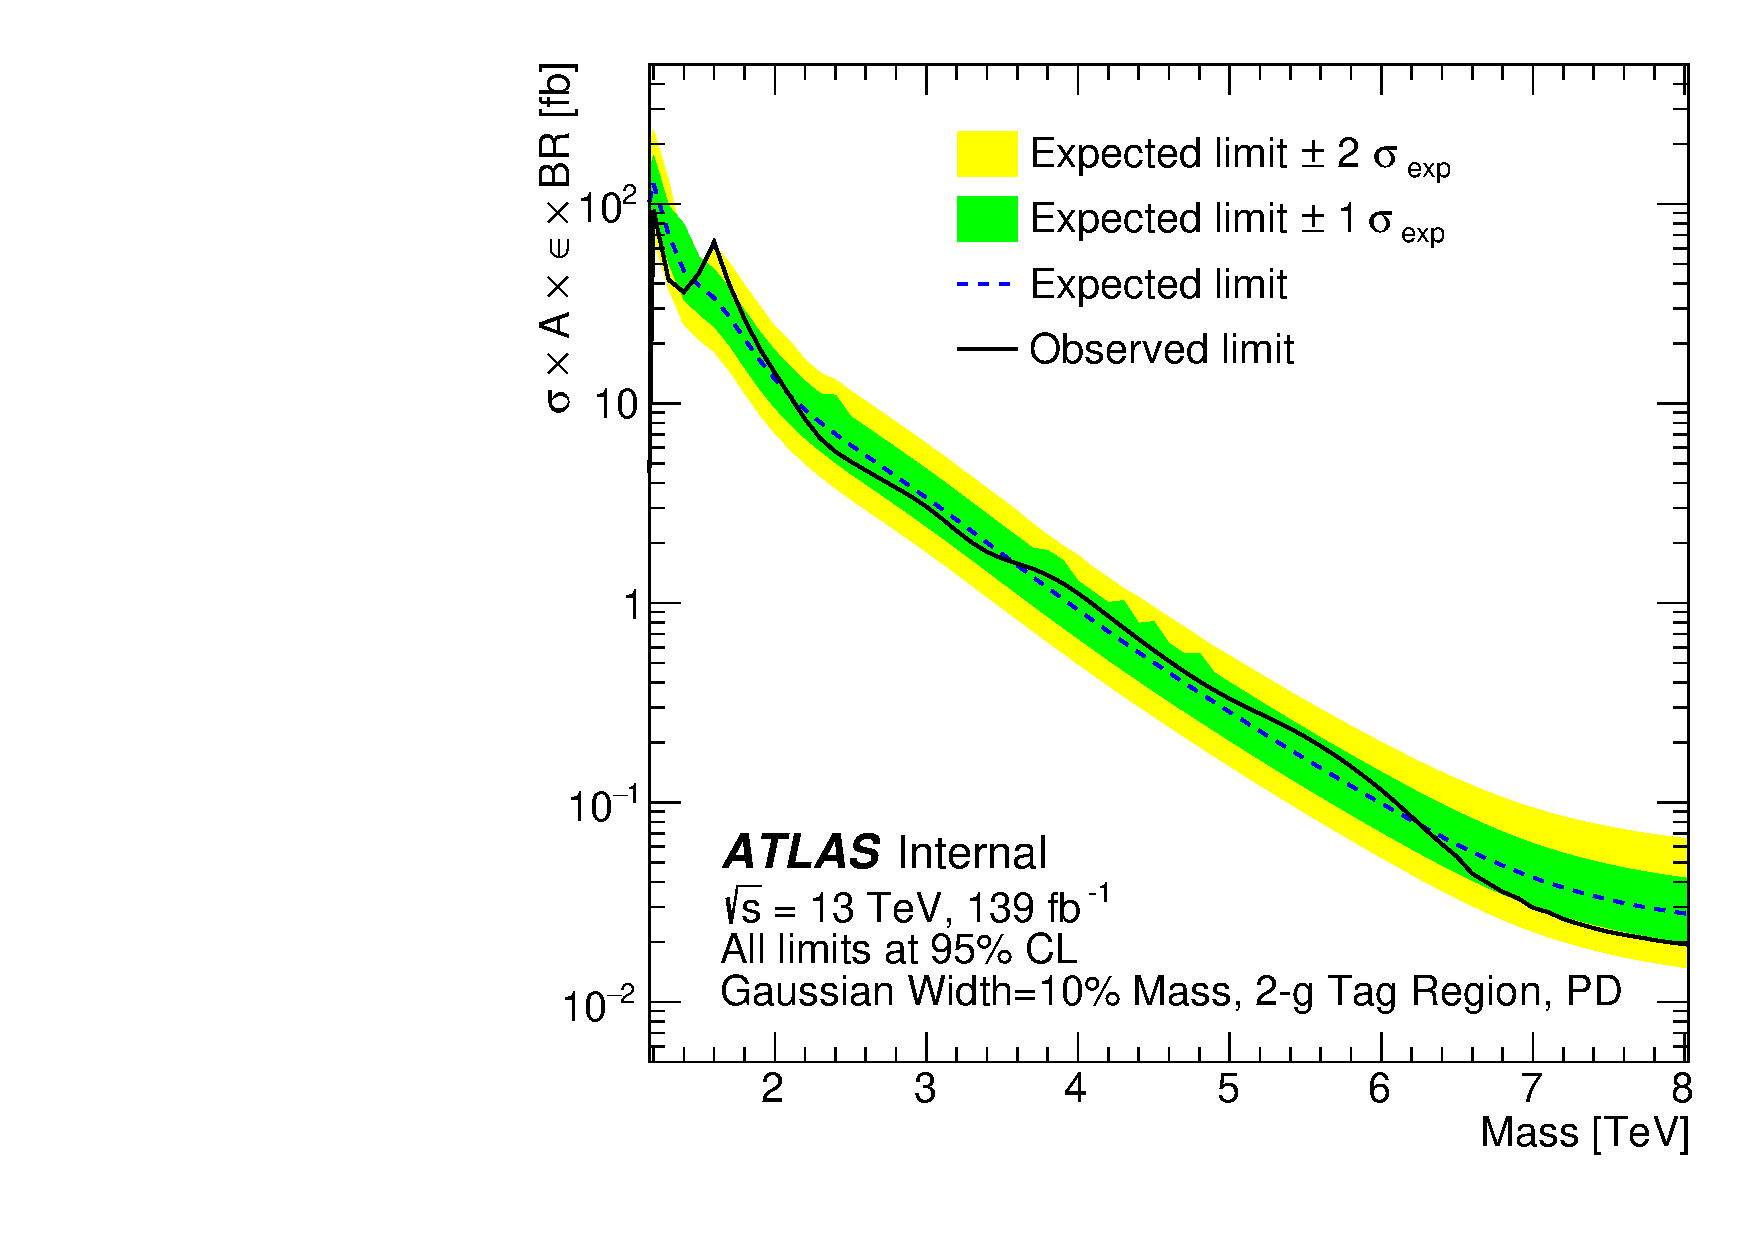
\includegraphics[width=0.4\textwidth]{fig/app-SignalIndependentLimits/Gauss_Limits_yStar0p8_Tag2_WidthPercent10_1200to8000_sigma.pdf}
            }
            \subfloat[15\% Width Gaussian Limits]{ 
%                \label{fig:SignalIndependentGaussianLimits_SubWidth15} % uncomment if label used. 
                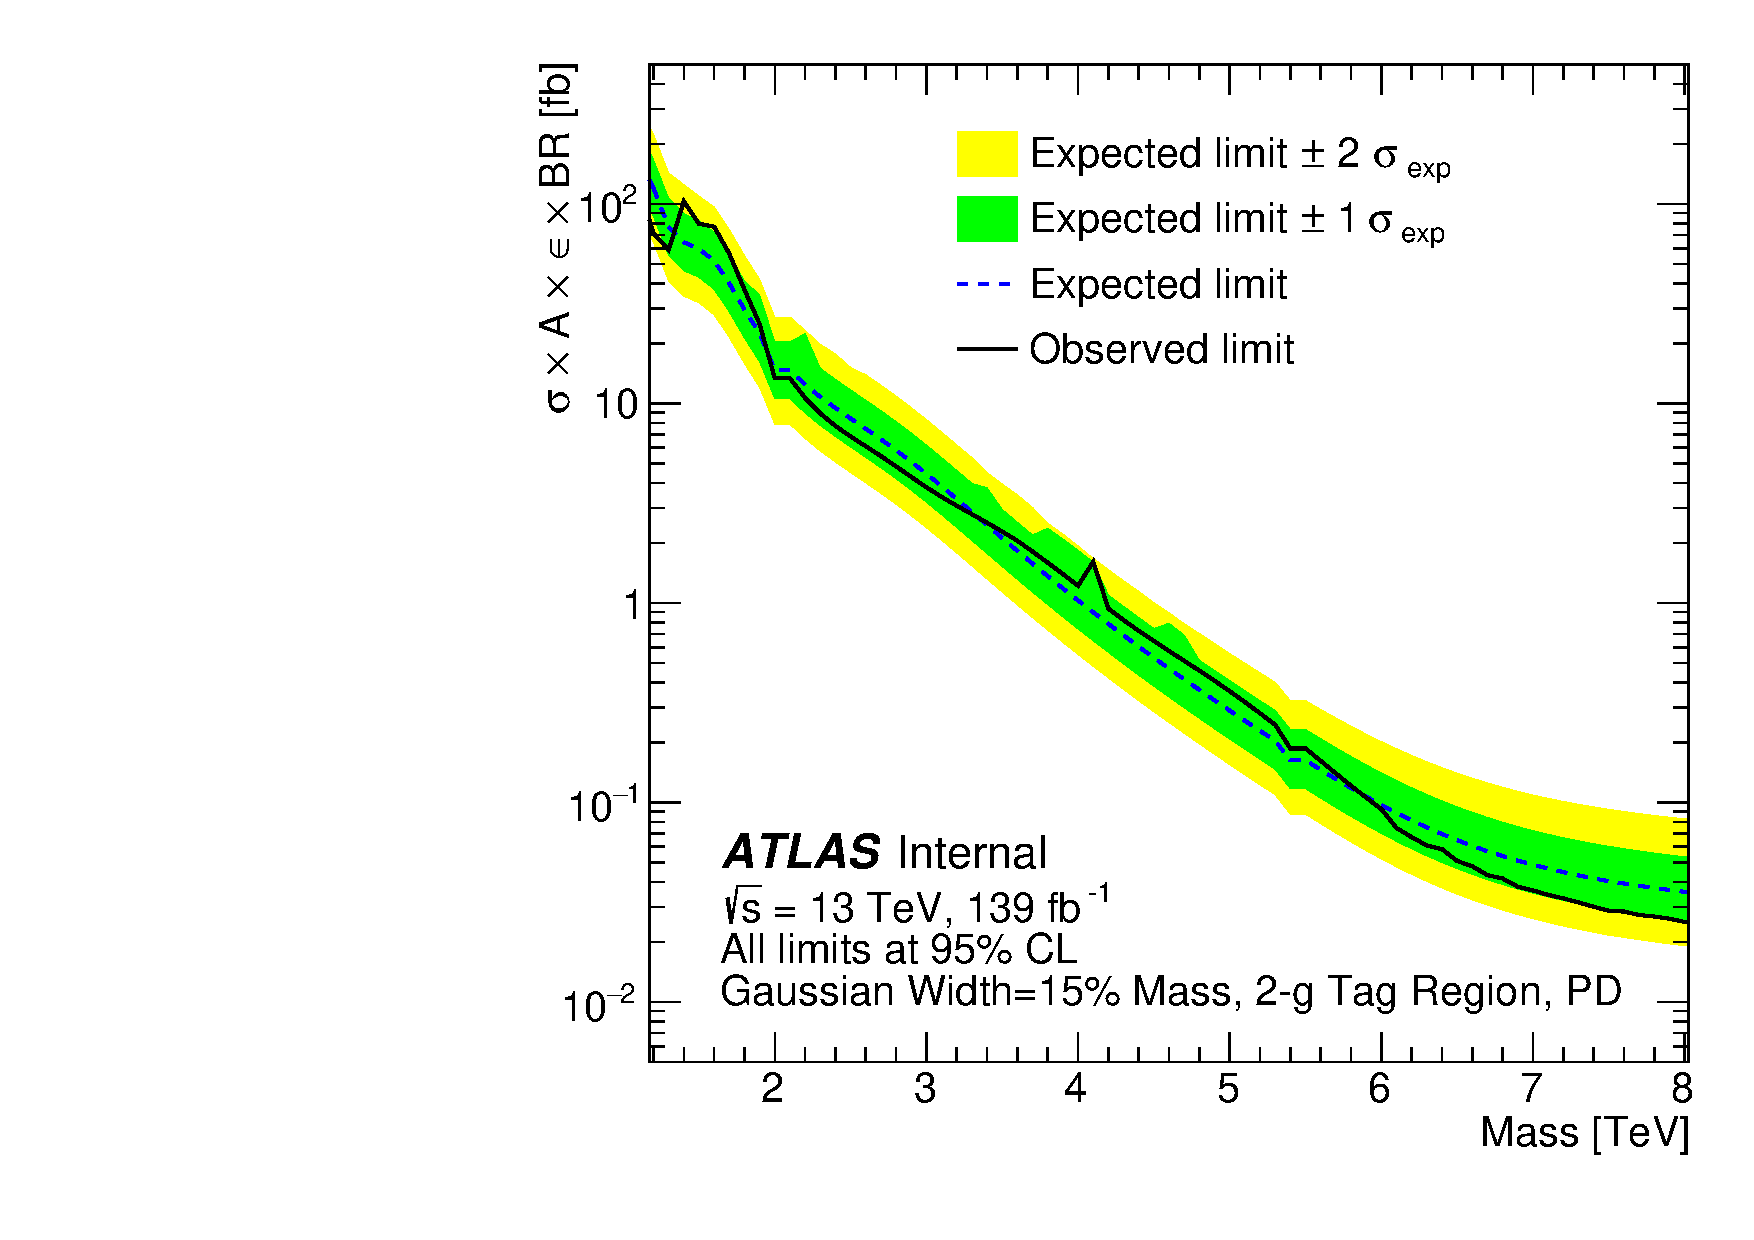
\includegraphics[width=0.4\textwidth]{fig/app-SignalIndependentLimits/Gauss_Limits_yStar0p8_Tag2_WidthPercent15_1200to8000_sigma.pdf}
            }
            \caption{Model-independent limits set in the 2-$g$ tagged $y^{*} < 0.8$ Signal Region using Gaussian resonances of varying widths from 0\% to 15\% of their peak position without systematics included using the full 139fb$^{-1}$ Run-2 dataset.}
            \label{fig:SignalIndependentGaussianLimits_2gYStar0p8}
        \end{figure}


